\documentclass{book}
\usepackage[UTF8]{ctex}
\usepackage[margin=1.5in]{geometry}
\usepackage{color}
\usepackage{amssymb}
\usepackage[many]{tcolorbox}    	% for COLORED BOXES (tikz and xcolor included)
\usepackage{setspace}               % for LINE SPACING
\usepackage{multicol}               % for MULTICOLUMNS
\usepackage{graphicx}
\usepackage{subfig}
\usepackage{float}

\usepackage{tikz,times,amsmath} %%分别是绘图宏包、字体宏包、数学公式宏包
%\usepackage{pgfplots} %% 这个宏包可以不加
\usepackage{tikz-3dplot} %%三维图形绘制需要的宏包
\usetikzlibrary{patterns}%%填充使用的宏包
\usetikzlibrary{3d,calc} %%3d 绘图及计算需要的库

\title{高中数学课本的``隐藏"知识}
\author{BiliBili: 小各的数学草稿; 琴剑天意}
\date{最后修改:\today}

\definecolor{main}{HTML}{5989cf}
\tcbset{
    sharp corners,
    colback = white,
    before skip = 0.2cm,    % add extra space before the box
    after skip = 0.5cm      % add extra space after the box
}                           % setting global options for tcolorbox

% You can copy any following box you like to your code.
\newtcolorbox{boxA}{
    fontupper = \bf,
    boxrule = 1.5pt,
    colframe = black % frame color
}

\newtcolorbox{boxB}{
    fontupper = \bf\color{main}, % font color
    boxrule = 1.5pt,
    colframe = main,
    rounded corners,
    arc = 5pt   % corners roundness
}

\begin{document}
    \maketitle
    \tableofcontents
    \chapter{序言}
    \section{编者序}
    感谢你翻开这本书.

    作为一个科研狗天天要用\LaTeX, 编这本书的目的是希望有一个自己的\LaTeX 作品, 练习之余也是将其作为一个艺术品来看, 同时也是出于对数学和计算机学的热爱. 不过在正式编排本书之前, 编者也曾想过是否有一个合适且高质量的数学内容整理, 来给同样热爱数学的大家发现数学之美. 编写这些内容, 首先选材难度是要有的, 过于简单枯燥没有思维深度则不是一个好书; 然而一味地追求难度更是不切实际, 结果只会适得其反, 甚至有``装逼''之嫌.

    同时编者又属于是INFP体质(虽然说这是一个刻板印象, 而且编者也不希望简单的将人格扁平化, 但是我还是喜欢拿MBTI来说事情), 喜欢有些``不切实际"的幻想, 想着有个非常完美的数学作品但是又懒得去动手, 整天想着做但是又是完美主义又怕做不好(是的, 我的内耗就这么简单).

    后来在BiliBili见到了一个专题, 来自于``小各的数学草稿''这位up主, 这就是本书的主题``高中课本的`隐藏'知识'', 这让编者感到相见恨晚, 选材独到, 源于课本又高于课本, 接地气的同时又充满了高级感. 唯一美中不足的是让编者强迫症犯的排版, 同时, 编者的梦想也算是有了一个着落, 在此感谢这位up主.

    也算是在这本书上倾注了很多心血, 包括使用Matplotlib绘制二维图片, 用\LaTeX 自带的 tikz 宏包绘制三维图片, 如果你使用电子介质阅读本书, 你将会发现得益于eps矢量图的特性, 书中的每一张图片中的每一个文字都可以复制, 每一条线都可以被无限放大而不失真. 至于绘制图片以及整本书的代码, 编者将会在使用说明章节中放置其开源地址, 本书完全免费自由, 但是我深深赞同费曼教授所言:``Knowledge isn't free. You have to pay attention." 从这个意义上看, 这本书却又并非完全“免费”. 对编者, 作者与读者都需要付诸大量的注意力, 只不过为了不辜负你为本书所付出的宝贵``注意力", 我会竭尽所能, 投入最大的``注意力"来完成本书的创作. 

    虽然编者没有光辉的学历背景, 在这人均985的互联网中显得有些自惭形秽, 但是学历只是其中的一个加分项而不是必须项; 只是很幸运, 这本书``找到''了热爱数学的你, 一同探究高中数学课本的知识; 希望你看完后, 你的水平能够更上一层楼.

    再次感谢你翻开这本书.

    {\hfill 琴剑天意}

    {\hfill \today}

    \section{本书资源}
    有请小各的数学草稿\dots\dots
    \section{使用说明}
    %本文原作者B站id: 小各的数学草稿, 本人仅作包括自己见解的\LaTeX 排版.

    下面是使用说明: 
    \begin{enumerate}
        \item 黑色的字迹是主要的过程
        \item \textcolor[rgb]{0.38,0.11,0.2}{紫色的字迹是拓展的知识或公式}
        \item \textcolor[rgb]{0.75,0.17,0.22}{红色的字迹是证明的较关键步骤}
        \item \textcolor[rgb]{0.11,0.65,0.52}{绿色的字迹是在课本上的相关出处}
        \item \textcolor[rgb]{0.13,0.47,0.72}{蓝色的字迹是编者加的用于框出题目}
        \item 证明题完毕后会带上一个象征性的$qed$符号代表结束$\blacksquare$
    \end{enumerate}
    \chapter{必修一}
    \section{\textcolor[rgb]{0.11,0.65,0.52}{P43, T9}}
    \begin{boxB}
        证明: 圆的面积大于与它具有相同周长的正方形的面积. 并据此说明, 人们通常把自来水管的横截面制成圆形而不是正方形的原因.
    \end{boxB}
    \doublespacing
    证明: 设两者周长均为$C$, 则圆的半径为$\displaystyle \frac{C}{2\pi}$, 而正方形边长为$\displaystyle \frac{C}{4}$, 故圆面积为$\displaystyle \pi(\frac{C}{2\pi})^2=\frac{C^2}{4\pi}$, 正方形面积$\displaystyle (\frac{C}{4})^2=\frac{C^2}{16}$.

    又因为$\displaystyle 4\pi < 4 \times 4 = 16$

    故在该条件下圆面积更大, 原因: 在横截面积一定情况圆耗费材料少.$\blacksquare$

    \textcolor[rgb]{0.38,0.11,0.2}{拓展引申: 周长相等的情况下, 圆的面积最大. (证明用到变分法)}
    \section{\textcolor[rgb]{0.11,0.65,0.52}{P43, T10}}
    \begin{boxB}
        已知$a$克糖水中含有$b$克糖$(a>b>0)$,再添加$m$克糖$(m>0)$(假设全部溶解), 糖水变甜了, 请将这一事实表示为不等式,并证明这个不等式成立.
    \end{boxB}

    本题涉及\textcolor[rgb]{0.38,0.11,0.2}{糖水不等式}:
    $$
    \frac{b}{a} < \frac{b+c}{a+c}, a>b>0, c>0
    $$

    证明过程:通过\textcolor[rgb]{0.75,0.17,0.22}{作差法}可得:
    $$
    \frac{b+c}{a+c} - \frac{b}{a} = \frac{(a-b)c}{a(a+c)}
    $$

    由$a>b$可得$a-b>0$, 而$a,b,c$均大于$0$, 故 $\displaystyle \frac{(a-b)c}{a(a+c)}>0. \blacksquare$

    编者有话说: 由于是糖水, 所以糖与糖水的比例肯定不会超过1,所以我们可以用1比较:
    $$
    1-\frac{b}{a}=\frac{a-b}{a},1-\frac{b+c}{a+c}=\frac{a-b}{a+c}
    $$
    $$
    \frac{a-b}{a}>\frac{a-b}{a+c}
    $$

    由此得证.$\blacksquare$

    \section{\textcolor[rgb]{0.11,0.65,0.52}{P75}}
    涉及\textcolor[rgb]{0.38,0.11,0.2}{狄利克雷函数}的相关问题:

    随着对微积分研究的深入, 18世纪末19世纪初, 入们对函数的认识向前推进了.德国数学家狄利克雷(P. G. L. Dirichlet, 1805—1859) 在1837年时提出: ``如果对于$z$ 的每一个值, $y$总有一个完全确定的值与之对应, 那么$y$是$z$的函数."这个定义较清楚地说明了函数的内涵. 只要有一个法则, 使得取值范围中的每一个$z$, 有一个确定的和它对应就行了, 不管这个法则是用公式还是用图象、表格等形式表示.例如, 狄利克雷函数, 即: 当自变量取有理数时, 函数值为1;当自变量取无理数时, 函数值为0.它只能用对应的语言予以表达.19世纪70年代以后, 随着集合概念的出现, 函数概念又进而用更加严谨的集合和对应语言表述, 这就是本节学习的函数概念.综上所述可知, 函数概念的发展与生产、生活以及科学技术的实际需要紧密相关, 而且随着研究的深入, 函数概念不断得到严谨化、精确化的表达, 这与我们学习函数的过程是一样的.

    这是\textcolor[rgb]{0.38,0.11,0.2}{狄利克雷函数}:
    $$
    f(x)=\begin{array}{l} 
            \left\{\begin{matrix} 
            1 \quad x \in \mathbb{Q} \\ 
            0 \quad x \in \mathbb{R} \setminus \mathbb{Q} \
          \end{matrix}\right.    
        \end{array} 
    $$

    \section{\textcolor[rgb]{0.11,0.65,0.52}{P87, T13}}
    \textcolor[rgb]{0.38,0.11,0.2}{对称性}和\textcolor[rgb]{0.38,0.11,0.2}{奇偶性}的关系.

    $f(x)$为奇函数表明关于$(0,0)$中心对称, $f(x)$为偶函数表明关于$x=0$对称.

    \begin{boxB}
        证明: $y=f(x)$的图象关于点$P(a,b)$成中心对称图形的充要条件是函数$y=f(x+a)-b$为奇函数.
    \end{boxB}

    \textcolor[rgb]{0.75,0.17,0.22}{充分性}:
        关于$(a,b)$中心対称$\Longrightarrow f(x)+f(2a-x)=2b\Longrightarrow f(x+a)+f(a-x)=2b$通过变形:$f(x+a)-b=-f(a-x)+b=-[f(a-x)-b]$满足其为奇函数$-f(x)=f(-x)$

    \textcolor[rgb]{0.75,0.17,0.22}{必要性}:
    $y=f(x+a)-b$奇函数$\Longrightarrow f(x+a)b=[f(a-x)-b]$通过变形可得到$f(x+a)+f(a-x)=2b$$\Longrightarrow$关于$(a,b)$中心对称. $\blacksquare$

    另外也有函数$y=f(x)$的图象关于$x=a$成轴对称的充要条件是函数$y=f(a+x)$为偶函数

    \section{\textcolor[rgb]{0.11,0.65,0.52}{P101, T8}}
    \begin{boxB}
        \begin{enumerate}
            \item 若$f(x)=ax+b$, $\displaystyle f(\frac{x_1x_2}{2})=\frac{f(x_1)+f(x_2)}{2}$.
            \item 若$g(x)=x^2+ax+b$则$\displaystyle f(\frac{x_1x_2}{2})\le \frac{g(x_1)+f(x_2)}{2}$.
        \end{enumerate}
    \end{boxB}
    本题实际上涉及了\textcolor[rgb]{0.38,0.11,0.2}{凹凸性}以及\textcolor[rgb]{0.38,0.11,0.2}{琴生不等式}的相关知识, 相关说明如下:
    \begin{enumerate}
        \doublespacing
        \item $\displaystyle f(\frac{x_1+x_2}{2})=a\cdot \frac{x_1+x_2}{2}+b, \frac{f(x_1)+f(x_2)}{2}=\frac{ax_1+b+ax_2+b}{2}=a\cdot \frac{x_1+x_2}{2}+b$.
        \item \textcolor[rgb]{0.75,0.17,0.22}{作差分析}: $\displaystyle g(\frac{x_1+x_2}{2})-\frac{g(x_1)+g(x_2)}{2}\\=(\frac{x_1+x_2}{2})^2+a\frac{x_1+x_2}{2}+b-\frac{x_1^2+ax_1+b+x_2^2+ax_2+b}{2}\\=-\frac{x_1^2-2x_1x_2+x_2^2}{4}=-\frac{(x_1-x_2)^2}{4}\le 0$.$\blacksquare$
    \end{enumerate}
    此处仅是解题并指出, 在选必二中会对其相关知识加以拓充补充.
    \section{\textcolor[rgb]{0.11,0.65,0.52}{P101, T12}}
    \begin{boxB}
        试讨论函数$\displaystyle y=x-\frac{1}{x}$的定义域, 值域, 单调性, 奇偶性, 并画出函数图像.
    \end{boxB}
    这是对勾函数所拓充出的函数, 我个人习惯说是双撇函数.由于$x=0$函数不存在, 定义域为$\{x|x\neq 0\}$而值域是$\mathbb{R}$, $y'=1+\frac{1}{x^2}>0$恒成立, 故函数在$(-\infty ,0)$和$(0,+\infty )$上单调递增;
        
    同时, $\displaystyle f(-x)=-x-\frac{1}{-x}=-x+\frac{1}{x}=-f(x)$为奇函数.
    \begin{figure}[htbp]
        \centering
        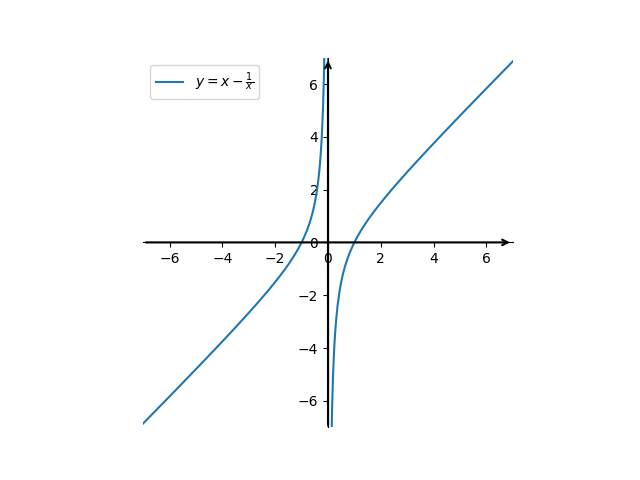
\includegraphics[width=0.5\textwidth]{img/sp.png}
        \caption{对撇函数}
    \end{figure}
    \section{\textcolor[rgb]{0.11,0.65,0.52}{P110, T10(2)}}
    \begin{boxB}
        当$n$越来越大时, $\displaystyle (1+\frac{1}{n})^{n}$的底数越来越小, 而指数越来越大, 那么$\displaystyle (1+\frac{1}{n})^{n}$是否也会越来越大? 有没有最大值?
    \end{boxB}
    本题涉及到一个重要极限$\displaystyle \lim_{x \to \infty} (1+\frac{1}{n} )^n=e$, 介绍一波$e$的由来;

    当你有$1$单位的本金并存进银行, 而年的利率为$r$, 如果我一年结算一次, 这样的话一年后就有了$(1+r)$单位的钱.

    如果我一年结算两次, 此时每年的收益率就相应的减为$\displaystyle \frac{r}{2}$, 第一期收益的产也被计入为第二期的本金, 因此一年就有$\displaystyle (1+\frac{r}{2})^2$单位的钱.如果一年分三期, 那么操作同样, 一年下来就有$\displaystyle (1+\frac{r}{3})^3$

    但一年分三期是比一年分两期要高的, 如果一年分的期次越高, 总收益$\displaystyle (1+\frac{r}{n})^n$, 也会越高. 但当$n\to \infty$时收益并不会趋于无穷, 它是有界的, 当$r=1$的时候便有$\displaystyle \lim_{x \to \infty} (1+\frac{1}{n} )^n=e$, 还有一般形式$\displaystyle \lim_{x \to \infty} (1+\frac{r}{n} )^n=e^r$. 

    来一波小小的应用:
    \begin{boxB}
        证明$e<3$.
    \end{boxB}
    证明: 由于$\displaystyle \lim_{x \to \infty} (1+\frac{1}{n} )^n=e$, $\displaystyle (1+\frac{1}{n} )^n$的形式可以使用二项式定理, 令$\displaystyle f(n)=(1+\frac{1}{n} )^n$:
    $$
    f(n)=(1+\frac{1}{n})^n=1+C_n^1\frac{1}{n}+C_n^2\frac{1}{n}+C_n^3\frac{1}{n}+\cdots +C_n^n\frac{1}{n^n}
    $$
    展开组合式可得:
    $$
    1+1+\frac{n(n-1)}{2!}\frac{1}{n^2}+\frac{n(n-1)(n-2)}{3!}\frac{1}{n^3}+\frac{n(n-1)(n-2)}{3!}\frac{1}{n^3}+\cdots +\frac{n(n-1)\cdots (n-n+1)}{n!}\frac{1}{n^n}
    $$
    初步化简得:
    $$
    f(n)=1+1+\frac{1}{2!}(1-\frac{1}{n})+\frac{1}{3!}(1-\frac{1}{n})(1-\frac{2}{n})+\cdots +\frac{1}{n!}(1-\frac{1}{n})(1-\frac{2}{n})(1-\frac{3}{n})\cdots (1-\frac{n-1}{n})
    $$
    当$n\ge 4$时, $n!=1\times2\times3\times4\times\cdots \times n>n(n-1)$
    所以: 
    $$
    f(n)<1+1+\frac{1}{2!}+\frac{1}{3!}+\frac{1}{3\times4}+\frac{1}{4\times5}+\cdots +\frac{1}{n(n-1)}
    $$
    进一步化简右式:
    $$
    f(n)<1+1+\frac{1}{1\times2}+\frac{1}{2\times3}+\frac{1}{3\times4}+\frac{1}{4\times5}+\cdots+\frac{1}{n(n-1)}
    $$
    右式裂项得:
    $$
    2+1-\frac{1}{2}+\frac{1}{2}-\frac{1}{3}+\frac{1}{3}-\cdots-\frac{1}{n} \le 3
    $$
    所以$e<3$.$\blacksquare$
    \section{\textcolor[rgb]{0.11,0.65,0.52}{P160, T6}}
    \begin{boxB}
        设$\displaystyle f(x)=\frac{e^x-e^{-x}}{2}$, $\displaystyle g(x)=\frac{e^x+e^{-x}}{2}$, 求证:\par
    \begin{enumerate}
        \item $[g(x)]^2-[f(x)]^2=1$
        \item $f(2x)=2f(x)g(x)$
        \item $g(2x)=[g(x)]^2+[f(x)]^2$
    \end{enumerate}
    \end{boxB}
        本题涉及\textcolor[rgb]{0.38,0.11,0.2}{双曲函数}的一些小性质, 其中$\displaystyle \sinh x = \frac{e^x-e^{-x}}{2}$, $\displaystyle \cosh x = \frac{e^x+e^{-x}}{2}$
    \begin{enumerate}
        \item $\displaystyle \cosh^2 x-\sinh^2x=(\cosh x+\sinh x)(\cosh x-\sinh x)\\=(\frac{e^x-e^{-x}}{2}+\frac{e^x+e^{-x}}{2})(\frac{e^x-e^{-x}}{2}-\frac{e^x+e^{-x}}{2})=\frac{2e^x}{2}\frac{2e^{-x}}{2}=e^x\cdot \frac{1}{e^x}=1$
        \item $\displaystyle \sinh 2x=\frac{e^{2x}-e^{-2x}}{2}, 2\sinh x \cosh x=2\cdot \frac{e^x-e^{-x}}{2}\cdot \frac{e^x+e^{-x}}{2}=\frac{e^{2x}-e^{-2x}}{2}$
        \item $\displaystyle \cosh 2x=\frac{e^{2x}+e^{-2x}}{2}, \cosh^2x+\sinh^2x=(\frac{e^x-e^{-x}}{2})^2+ (\frac{e^x+e^{-x}}{2})^2\\=\frac{e^{2x}+e^{-2x}}{2}$. $\blacksquare$
    \end{enumerate}

    还有其它性质:$\cosh x$是偶函数, $\sinh x$是奇函数. 
        
    另外还有由\textcolor[rgb]{0.75,0.17,0.22}{基本不等式}可知: $\displaystyle \sinh x=\frac{e^x+e^{-x}}{2} \ge \frac{2\sqrt{e^xe^{-x}}}{2}=1$

    \textcolor[rgb]{0.38,0.11,0.2}{回看问题1,$x^2+y^2=1$代表单位圆$x=\cos \theta, y=\sin \theta$, 而$x^2-y^2=1$代表单位双曲线$x=\cosh t, y=\sinh t$.}
    
    \begin{figure}[htbp]    % 常规操作\begin{figure}开头说明插入图片
        % 后面跟着的[htbp]是图片在文档中放置的位置, 也称为浮动体的位置, 关于这个我们后面的文章会聊聊, 现在不管, 照写就是了
          \centering            % 前面说过, 图片放置在中间
          \subfloat[双曲正弦函数$y=\sinh x$]   % 第一张子图的下标(注意: 注释要写在[]中括号内)
          {
              \label{fig:subfig1}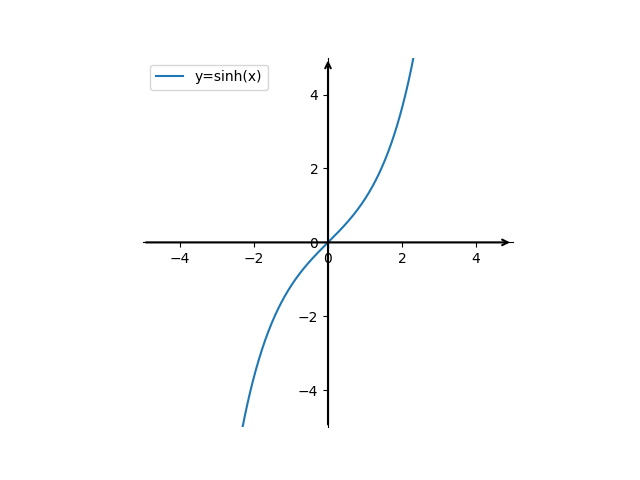
\includegraphics[width=0.4\textwidth]{img/sinhx.png}
              % \label{}命令为每个子图添加标签, 方便在正文中引用. 如果你不需要引用的话, 也可以不加这个命令, 写法在下面有: 
              % \label{}命令的{}内第一个{}中的内容fig:subfig1就是你插入的这张子图的标签, 注意每个标签都不能一样, 要用合适的编号去区分, 比如1、2、3......
              % \label{}命令中{}内\includegraphics[]{}就是真正插入图片的命令, []中的是图片的一些参数, {}就是图片的相对路径
              % width=0.4\textwidth 就是设置图片的大小, 这里设置的是文档宽度(\textwidth)的0.4倍, 在设置时注意不要超宽, 不然会报错, 大家多设置几个数尝试一下就能理解了
          }
          \subfloat[双曲余弦函数$y=\cosh x$]
          {
              \label{fig:subfig2}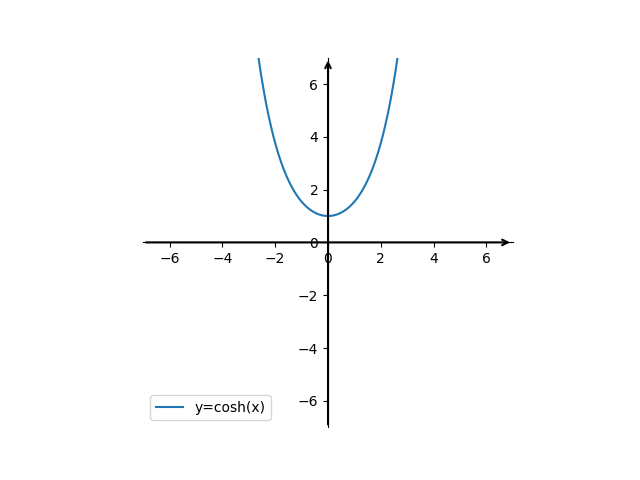
\includegraphics[width=0.4\textwidth]{img/coshx.png}
          }
          \caption{双曲函数}    % 整个图片的说明, 注释写在{}内
          \label{fig:subfig_1}            % 整个图片的标签编号, 注意这里跟子图是一样的道理, 标签不能重复 
        \end{figure}
    \section{\textcolor[rgb]{0.11,0.65,0.52}{P225例8, P226T4, 5}}
    \begin{boxB}
        \begin{enumerate}
            \item 证明: $\displaystyle \sin a\cos b=\frac{1}{2}[\sin(a+b)+\sin(a-b)]$
            \item 证明: $\displaystyle \sin \theta + \sin \varphi = 2\sin\frac{\theta+\varphi}{2}\cos\frac{\theta-\varphi}{2}$
        \end{enumerate}
    \end{boxB}
    解答过程如下:

    \begin{enumerate}
        \item $$\sin (a+b)=\sin a\cos b+\sin b \cos a, \sin (a-b)=\sin a\cos b-\sin b \cos a$$\textcolor[rgb]{0.75,0.17,0.22}{两式相加}$$\sin(a+b)+\sin(a-b)=2\sin a\cos b$$两边同除2得证. $\blacksquare$
        \item 根据上述结论得:$$\sin(a+b) +\sin(a-b)=2\sin a\cos b$$\textcolor[rgb]{0.75,0.17,0.22}{令$a+b=\theta$, $a-b=\varphi$,则有$\displaystyle a=\frac{\theta+\varphi}{2},b=\frac{\theta-\varphi}{2}$}, 代入便可得证. $\blacksquare$
    \end{enumerate}

    其它的\textcolor[rgb]{0.38,0.11,0.2}{积化和差}:
    \begin{enumerate}
        \item $\displaystyle \sin a\sin b=-\frac{1}{2}[\cos(a+b)-\cos(a-b)]$
        \item $\displaystyle \cos a\sin b=\frac{1}{2}[\sin(a+b)-\sin(a-b)]$
        \item $\displaystyle \cos a\cos b=\frac{1}{2}[\cos(a+b) +\cos(a-b)]$
    \end{enumerate}

    其它的\textcolor[rgb]{0.38,0.11,0.2}{和差化积}:

    \begin{enumerate}
        \item $\displaystyle \sin \theta-\sin \varphi=2\cos\frac{\theta+\varphi}{2}\sin\frac{\theta-\varphi}{2}$
        \item $\displaystyle \cos \theta+\cos \varphi=2\cos \frac{\theta+\varphi}{2} \cos \frac{\theta-\varphi}{2}$
        \item $\displaystyle \cos \theta-\cos \varphi=-2\sin \frac{\theta+\varphi}{2} \sin \frac{\theta-\varphi}{2}$
    \end{enumerate}

    \section{\textcolor[rgb]{0.11,0.65,0.52}{P250 阅读与思考}}
    
    \begin{center}
        振幅、周期、频率、相位
    \end{center}

    人体就是一个包合各种周期运动的生物体, 医学上把周期为24小时的生理运动称为中周期运动, 如血压、血糖浓度的变化; 小于24小时的叫短周期运动,  如心跳、脉搏每分50$\sim$70次、呼吸每分16$\sim$24次; 大于24小时的叫长周期运动, 如人的情绪、休力、智力等. 
    
    声音中也包含着正弦函数, 声音是由于物体的振动产生的能引起听觉的波. 每一个音都是由纯音合成的, 纯音的数学模型是函数 $y=A\sin \omega t$有四要素:  音调、响度、音长和音色, 这都与正弦函数的参数有关, 响度与振幅有关, 即与 声波的能量有关, 振幅越大, 响度越大, 音长也与振幅有关, 声音消失过程是由 于声波在传播过程中受阻尼振动, 系统的机械能随时间逐渐减小, 振动的振幅也 逐渐减小, 音调与声波的振动频率是有关的, 频率低的声音低沉, 频率高的声音尖
    利.像我们平时听到的乐音不只是一个音在响, 而是许多个音的结合, 称为复合音.  复合音的产生是因为发声体在全段振动, 产生频率为/的基音的同时, 其各部分,  如二分之一、三分之一、四分之一部分也在振动, 产生的频率恰好是全段振动频率的倍数, 如2$f$, 3$f$, 4$f$等.这些音叫谐音, 因为其振幅较小, 我们一般不易单独听出来所以我们听到的声音的函数是$\displaystyle y=\sin x+\frac{1}{2}\sin 2x+\frac{1}{3}\sin 3x+\frac{1}{4}\sin 4x+\cdots$

    音色一般是由基音和谐音的综合作用所决定的, 不同乐器、不同人发出的音调可以相同, 但音色不同, 人们由此分辨出不同的声音.
    
    周期函数产生了美妙的音乐!

    \section{\textcolor[rgb]{0.11,0.65,0.52}{P256, T26}}
    英国数学家泰勒发现了如下公式\textcolor[rgb]{0.38,0.11,0.2}{(泰勒展开)}:
    $$
    \sin x = x - \frac{x^3}{3!}+\frac{x^5}{5!}-\frac{x^7}{7!}+\cdots,
    \cos x = 1-\frac{x^2}{2!}+\frac{x^4}{4!}-\frac{x^36}{6!}+\cdots
    $$

    其中$n!=1\times2\times3\times\cdots\times n$

    我们可以用\textcolor[rgb]{0.75,0.17,0.22}{物理的角度}来理解该公式:

    \begin{enumerate}
        \item 如果以速度$v$匀速直线推木块, 则关系式为$f(t)=x_0+vt$, 其中$x$是初位置, 此时求导就可以得到瞬时速度$f'(t)=v$
        \item 如果以加速度$a$恒定(不为0)推木块, 则如上操作可知$f''(t)=a$, 此时对其逆向推理可得$f'(t)=v+at$,再对$\displaystyle f'(t)$使用$\displaystyle f(t) =x+vt+\frac{1}{2}at^2$
        \item 如果此时加速度的变化是恒定的, 即逆向推理可得$\displaystyle f''(t)=a+a_xt$, (斜率对$a$的变化为$a_x$)$\displaystyle f'(t)=v+at+\frac{1}{2}a_xt^2\Longrightarrow f(t)=x+vt+\frac{1}{2}at^2+\frac{1}{6}a_xt^2$, 如此操作下去有: $$f(t)=x_0+x_1t+\frac{1}{2}x_2t^2+\frac{1}{6}x_3t^3+\cdots+\frac{1}{n!}x_nt^n$$用$x-x_0$代替$t$有:$$f(x)=f(x_0)+\frac{f'(x_0)}{1!}(x-x_0)+\frac{f''(x_0)}{2!}(x-x_0)^2+\frac{f'''(x_0)}{3!}(x-x_0)^3+\cdots$$
    \end{enumerate}

    \textcolor[rgb]{0.38,0.11,0.2}{泰勒公式:} $$f(x)=f(x_0)+\frac{f'(x_0)}{1!}(x-x_0)+\frac{f''(x_0)}{2!}(x-x_0)^2+\frac{f'''(x_0)}{3!}(x-x_0)^3+\cdots$$

    令$x_0=0$此时$\displaystyle f(x)=f(0)+\frac{f'(0)}{1!}x+\frac{f''(0)}{2!}x^2+\frac{f'''(0)}{3!}x^3+\cdots$(在0处开始拟合)

    如果令$\displaystyle f(x)=e^x$有$\displaystyle e^x=e^0+e^0x+\frac{1}{2}e^0x^2+\cdots=1+x+\frac{x^2}{2!}+\frac{x^3}{3!}$

    其它的泰勒公式也可以同样得到, 这里就直接给到大家了:

    \begin{enumerate}
        \item $\displaystyle \ln (x+1)=x-\frac{x^2}{2}+\frac{x^3}{3}-\cdots$
        \item $\displaystyle \sqrt{x+1}=1+\frac{1}{2}x-\frac{1}{8}x^2+\frac{1}{16}x^3-\cdots$
        \item $\displaystyle \sin x = x-\frac{x^3}{3!}+\frac{x^5}{5!}-\frac{x^7}{7!}+\cdots$
        \item $\displaystyle \cos x=1-\frac{x^2}{2!}+\frac{x^4}{4!}-\frac{x^6}{6!}+\cdots$
    \end{enumerate}

    其实简单来说泰勒公式就是在某点($x_0$)附近开始拟合, 随着右边多项式的增加从而让拟合效果越来越好.

    大家也可以自行根据得到的普遍的公式推导其它函数的泰勒公式.
    \chapter{必修二}
    \section{\textcolor[rgb]{0.11,0.65,0.52}{P9}}
    \begin{boxB}
        证明\textcolor[rgb]{0.38,0.11,0.2}{绝对值三角不等式}: $$
        ||\overrightarrow{a}|-|\overrightarrow{b}||\le|\overrightarrow{a}+\overrightarrow{b}|\le|\overrightarrow{a}|+|\overrightarrow{b}|
        $$
    \end{boxB}

    让$\overrightarrow{a}$与$\overrightarrow{b}$转化为共起点的,形成一个角度$\theta$, 则$\overrightarrow{a}$与$\overrightarrow{b}$可利用平行四边形法则绘制如图3所示:
    \begin{figure}[htbp]
        \centering
        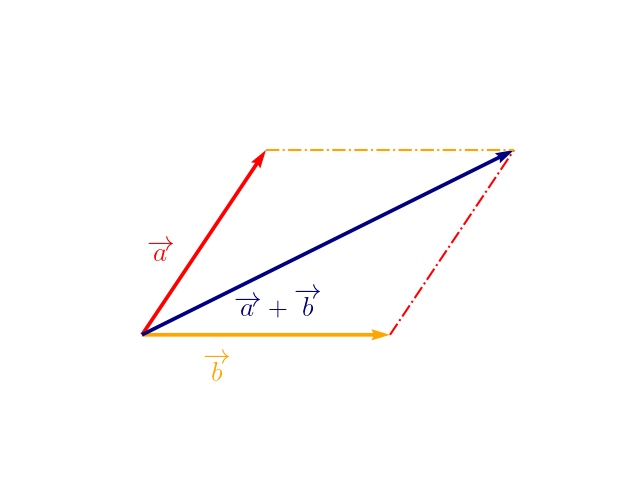
\includegraphics[width=0.5\textwidth]{img/vector.png}
        \caption{向量证明}
    \end{figure}

    $\displaystyle |\overrightarrow{a}+\overrightarrow{b}|$可表示这条对角线的长度, 而$|\overrightarrow{a}|+|\overrightarrow{b}|$可表示$\overrightarrow{a}$与$\overrightarrow{b}$同向时的长度, $|\overrightarrow{a}|-|\overrightarrow{b}|$为$\overrightarrow{a}$与$\overrightarrow{b}$反向时候的长度.

    在$|\overrightarrow{a}|+|\overrightarrow{b}|$构成三角形时\textcolor[rgb]{0.75,0.17,0.22}{第三边小于两边之和且大于两边之差}, 当面仅当两尚量同向或者两向量中存在0向量的取到右边等号, 当且仅当两向量异号或者两向量存在0向量时取到左边等号.$\blacksquare$

    \section{\textcolor[rgb]{0.11,0.65,0.52}{P6 例1}}

    如图$\overrightarrow{OA}$与$\overrightarrow{OB}$不共线, 且$\overrightarrow{AP}=t\overrightarrow{AB}, (t\in \mathbb{R})$, 用$\overrightarrow{OA},\overrightarrow{OB}$来表示$\overrightarrow{OB}$

    因为$\overrightarrow{PA}=t\overrightarrow{AB}$, 所以$\overrightarrow{OA}+\overrightarrow{AP}=\overrightarrow{OA}+t\overrightarrow{AB}=\overrightarrow{OA}+t(\overrightarrow{OB}-\overrightarrow{OA})=(1-t)\overrightarrow{OA}-t\overrightarrow{OB}$

    \textcolor[rgb]{0.38,0.11,0.2}{平面向量基本共线定理}: $\overrightarrow{OP}=a\overrightarrow{OA}+b\overrightarrow{OB},(a+b=1)$

    拓展一波更一般结论, 还是用刚刚那张图,如果说$AB:CB=a:b$, 则$\displaystyle \overrightarrow{OB}=\frac{a}{a+b}\overrightarrow{OA}+\frac{b}{a+b}\overrightarrow{OP}$(大家可以用上面的方法自行推导一下)

    如果此时$\overrightarrow{OP}=a\overrightarrow{OA}+b\overrightarrow{OB}$, 此时$a+b\neq 1$这时候是一般的\textcolor[rgb]{0.38,0.11,0.2}{等和线定理}, 此时可先假设$a+b=x$

    然后如图 5.b 操作即可:
    \begin{figure}[htbp]    % 常规操作\begin{figure}开头说明插入图片
        % 后面跟着的[htbp]是图片在文档中放置的位置, 也称为浮动体的位置, 关于这个我们后面的文章会聊聊, 现在不管, 照写就是了
          \centering            % 前面说过, 图片放置在中间
          \subfloat[书本图]   % 第一张子图的下标(注意: 注释要写在[]中括号内)
          {
              \label{fig:subfig1}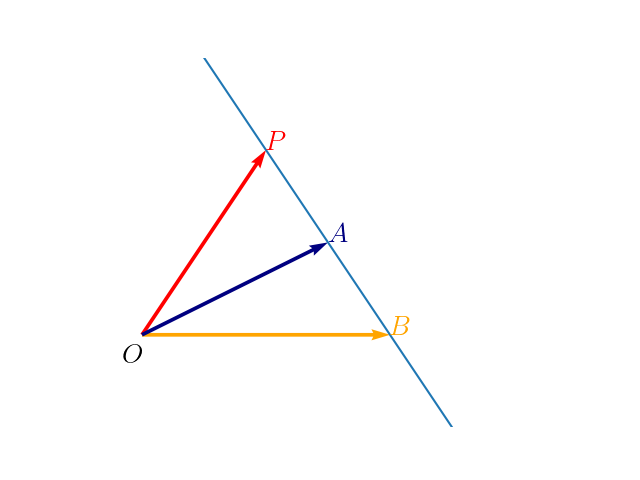
\includegraphics[width=0.4\textwidth]{img/equal_line.png}
              % \label{}命令为每个子图添加标签, 方便在正文中引用. 如果你不需要引用的话, 也可以不加这个命令, 写法在下面有: 
              % \label{}命令的{}内第一个{}中的内容fig:subfig1就是你插入的这张子图的标签, 注意每个标签都不能一样, 要用合适的编号去区分, 比如1、2、3......
              % \label{}命令中{}内\includegraphics[]{}就是真正插入图片的命令, []中的是图片的一些参数, {}就是图片的相对路径
              % width=0.4\textwidth 就是设置图片的大小, 这里设置的是文档宽度(\textwidth)的0.4倍, 在设置时注意不要超宽, 不然会报错, 大家多设置几个数尝试一下就能理解了
          }
          \subfloat[倍率等和线图]
          {
              \label{fig:subfig2}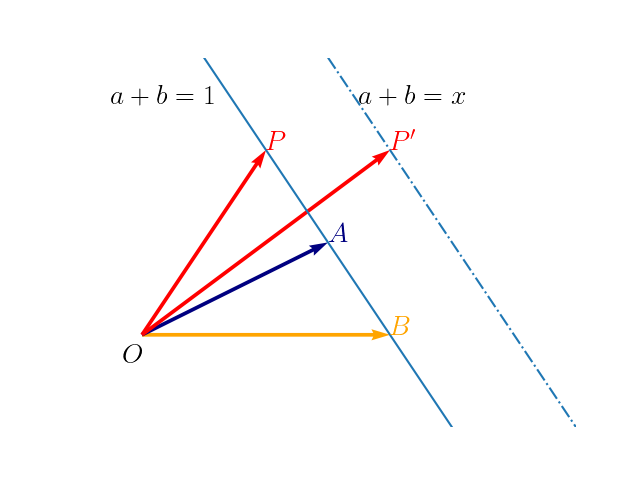
\includegraphics[width=0.4\textwidth]{img/eq_line_2.png}
          }
          \caption{等和线定理}    % 整个图片的说明, 注释写在{}内
          \label{fig:subfig_1}            % 整个图片的标签编号, 注意这里跟子图是一样的道理, 标签不能重复 
        \end{figure}

        做题步骤遵循以下步骤:
        \begin{enumerate}
            \item 找到它们所在位置;
            \item 在$P$点上做$AB$的平行线;
            \item 根据相似可得$\displaystyle x=\frac{OD}{OC}$
        \end{enumerate}

        \section{\textcolor[rgb]{0.11,0.65,0.52}{P33, 探究}}
        
        \begin{boxB}
            定比分点公式

            线段$P_1P_2$的端点$P_1P_2$的坐标分别为$(x_1,y_1)$, $(x_2,y_2)$, $P$是直线$P_1,P_2$上的一点, 当$P_1P_2=\varphi P_1P_2$时, 求点$P$的坐标.
        \end{boxB}
        设$P$点坐标$(x,y)$, 则有$$\overrightarrow{P_1P}=\varphi \overrightarrow{PP_2}\Longrightarrow (x-x_1,y-y_1)=\varphi(x_2-x, y_2-y)$$

        则有两式: $$x-x_1=\varphi (x_2-x),y-y_1=\varphi (y_2-y)$$

        解得:$$x=\frac{x_1+\varphi x_2}{1+\varphi},y=\frac{y_2+\varphi y_2}{1+\varphi}$$
        
        故$\displaystyle P(\frac{x_1+\varphi x_2}{1+\varphi},\frac{y_1+\varphi y_2}{1+\varphi})$. $\blacksquare$

        \section{\textcolor[rgb]{0.11,0.65,0.52}{P37, T16}}
        \begin{boxB}
            用向量方法证明: 对于任意的$a,b,c,d \in \mathbb{R}$恒有不等式$$(ac+bd)^2\le(a^2+b^2)(c^2+d^2)$$
            当且仅当$\displaystyle \frac{a}{c}=\frac{b}{d}$等号成立.
        \end{boxB}

        本题实际上是证明\textcolor[rgb]{0.38,0.11,0.2}{二维的柯西不等式}

        证明: 构造向量$\overrightarrow{a}=(a,b),\overrightarrow{b}=(c,d)$其夹角为$\theta$由$\cos \theta \in [-1,1]$可知$\cos ^2 \theta \le 1$则有$$\cos ^2 \theta=\left (\frac{\overrightarrow{a}\cdot \overrightarrow{b}}{|\overrightarrow{a}|\cdot |\overrightarrow{b}|}\right ) ^2=\left ( \frac{ac+bd}{\sqrt{a^2+b^2}\cdot \sqrt{c^2+d^2}} \right )^2 \le 1$$
        解得$$(ac+bd)^2 \le (a^2+b^2)(c^2+d^2)$$
        由\textcolor[rgb]{0.38,0.11,0.2}{柯西不等式}可引申出\textcolor[rgb]{0.38,0.11,0.2}{二维的权方和不等式}$$\frac{x_1^2}{y_1}+\frac{x_2^2}{y_2}\ge \frac{(x_1+x_2)^2}{y_1+y_2}$$
        令$\displaystyle a^2=\frac{x_1^2}{y_1},b^2\frac{x_2^2}{y_2},c^2=y_1,d^2=y_2$
        $$\left ( \frac{x_1^2}{y_1}+\frac{x_2^2}{y_2} \right )(y_1+y_2)\ge \left ( \frac{x_1}{\sqrt{y_1}}\sqrt{y_1}+\frac{x_2}{\sqrt{y_2}}\sqrt{y_2} \right )=(x_1+x_2)^2$$
        当且仅当$\displaystyle \frac{x_1}{y_1}=\frac{x_2}{y_2}$等号成立.$\blacksquare$
        \section{\textcolor[rgb]{0.11,0.65,0.52}{P39, 例2}}
        已知图5有$\overrightarrow{AC}=\overrightarrow{AB}+\overrightarrow{BC},\overrightarrow{DB}=\overrightarrow{AB}-\overrightarrow{BC}$, 则有$$\overrightarrow{AC}^2=\overrightarrow{AB}^2+\overrightarrow{BC}^2+2\overrightarrow{AB}\cdot \overrightarrow{BC},\overrightarrow{DB}^2=\overrightarrow{AB}^2+\overrightarrow{BC}^2-2\overrightarrow{AB}\cdot \overrightarrow{BC}$$
        \textcolor[rgb]{0.75,0.17,0.22}{两式相加}有$$AC^2+BD^2=2(AB^2+AD^2)$$
        \begin{figure}[htbp]
            \centering
            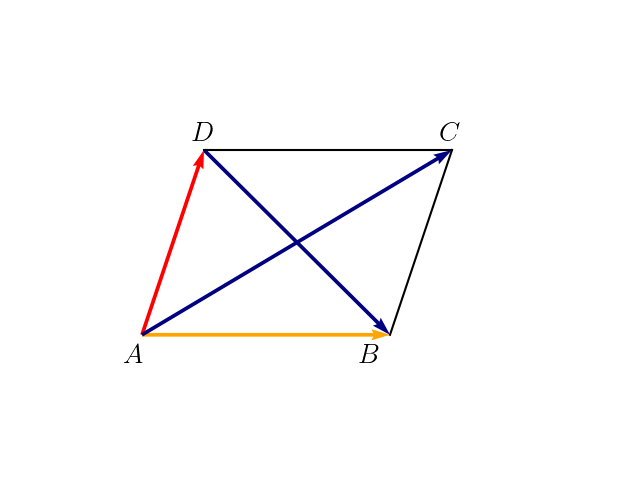
\includegraphics[width=0.5\textwidth]{img/PolarizationIdentity.png}
            \caption{平行四边形性质}
        \end{figure}
        此为平行四边形的性质.

        类似操作即可得到\textcolor[rgb]{0.38,0.11,0.2}{极化恒等式}: 

        如图6, 在$\triangle ABC$中, $D$为$BC$求证$\overrightarrow{AB}\cdot \overrightarrow{BC}=|AD|^2-|BD|^2$
        \begin{figure}[htbp]
            \centering
            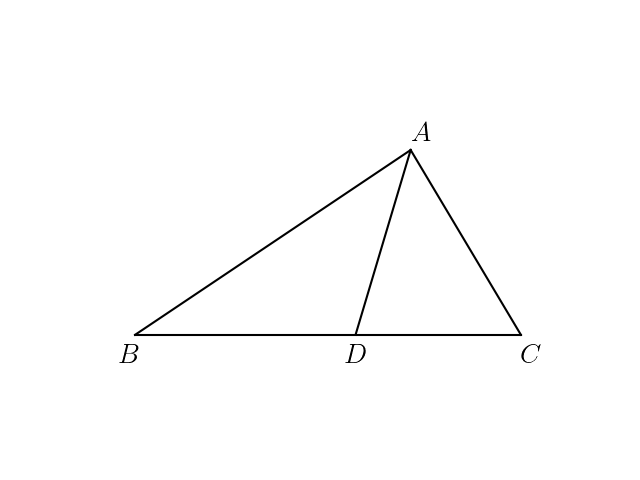
\includegraphics[width=0.5\textwidth]{img/PolarizationIdentity_p.png}
            \caption{极化恒等式}
        \end{figure}
        \begin{equation}
            \overrightarrow{AD}=\frac{1}{2} \left ( \overrightarrow{AB}+\overrightarrow{AC} \right )\Longrightarrow |\overrightarrow{AD}|^2=\frac{1}{4}\left ( \overrightarrow{AB}^2+\overrightarrow{AC}^2+2\overrightarrow{AB}\cdot \overrightarrow{AC} \right )
        \end{equation}

        \begin{equation}
            \overrightarrow{DB}=\frac{1}{2} \left ( \overrightarrow{AB}+\overrightarrow{AC} \right )\Longrightarrow |\overrightarrow{DB}|^2=\frac{1}{4}\left ( \overrightarrow{AB}^2-\overrightarrow{AC}^2+2\overrightarrow{AB}\cdot \overrightarrow{AC} \right )
        \end{equation}

        (1) - (2) 得:
        $$
        \overrightarrow{AB}\cdot \overrightarrow{AC}=|AD|^2-|BD|^2
        $$
        证毕.$\blacksquare$
        \section{\textcolor[rgb]{0.11,0.65,0.52}{P54, T20; P55$\sim$56}}
        \begin{boxB}
            证明: \textcolor[rgb]{0.38,0.11,0.2}{海伦公式}
            $$S_{\triangle ABC}=\sqrt{p(p-a)(p-b)(p-c)},p=\frac{a+b+c}{2}$$
        \end{boxB}
        由余弦定理得:
        $$\cos C=\frac{a^2+b^2-c^2}{2ab}$$
        由勾股定理得:
        $$\sin C = \sqrt{1-\cos^2 C}$$
        则$S_{\triangle ABC}$可表示为:
        $$\frac{1}{2}ab\sin C=\frac{1}{2}ab\sqrt{1-\left( \frac{a^2+b^2-c^2}{2ab}\right)^2}=\frac{1}{4}\sqrt{\left(2ab\right)^2-\left( a^2+b^2-c^2 \right)^2}$$
        将上式进一步化简:
        $$\frac{1}{4}\sqrt{\left( 2ab+a^2+b^2-c^2 \right)\left( 2ab-a^2-b^2+c^2 \right)}$$
        最后得到:
        $$\frac{1}{4}\sqrt{\left( a+b+c \right)\left( b+c-a \right)\left( c+a-b \right)\left( a+b-c \right)}$$
        又$\displaystyle p=\frac{a+b+c}{2}$对其变形有$\displaystyle \frac{1}{2}(b+c-a)=p-a,\frac{1}{2}(a+c-b)=p-b,\frac{1}{2}(a+b-c)=p-c$
        可得到海伦公式:
        $$
        S_{\triangle ABC}=\sqrt{p(p-a)(p-b)(p-c)},p=\frac{a+b+c}{2} .\blacksquare
        $$
        
        与其等价的为\textcolor[rgb]{0.38,0.11,0.2}{秦九韶公式}: 
        $$S_{\triangle ABC}=\sqrt{\frac{1}{4}\left[ a^2c^2-\left( \frac{c^2+a^2-b^2}{2} \right)^2 \right]}$$
        \section{\textcolor[rgb]{0.11,0.65,0.52}{P82}}
        这里涉及了\textcolor[rgb]{0.38,0.11,0.2}{代数基本定理}与\textcolor[rgb]{0.38,0.11,0.2}{较高次方程的韦达定理}:
        \begin{boxB}
            代数基本定理: 任何一个一元复系数多项式方程都至少有一个复数根
        \end{boxB}
        关于较高次方程的韦达定理的基本事实是: 任何一个一元复系数多项式方程均可表示为$X-x_n$的形式, 下面就是式子的描述:
        $$a_nX^n+a_{n-1}X^{n-1}+a_{n-2}X^{n-2}+a_1X=a_n(X-x_1)(X-x_2)(X-x_3)\cdots (X-x_n)$$
        简写为:
        $$\sum_{i=1}^{n} a_nX^{n}=a_n\prod_{i=1}^{n}\left ( X-x_n \right ) $$

        简单引入: 一元三次方程$a_3x^3+a_2x^2+a_1x+a_0=0,(a_3\neq0)$在复数集$\mathbb{C}$的根为$x_1,x_2,x_3$, 对其变形可得$a_3(x-x_1)(x-x_2)(x-x_3)=0$, 则有$a_3x^3-a_3(x_1+x_2+x_3)x^2+a_3(x_1x_2+x_2x_3+x_1x_3)x-a_3x_1x_2x_3=0$

        \textcolor[rgb]{0.75,0.17,0.22}{对比两个式子}有:
        $$
        \left\{\begin{matrix} 
            \displaystyle x_1+x_2+x_3=-\frac{a_2}{a_3}  \\  
            \displaystyle x_1x_2+x_2x_3+x_1x_3=\frac{a_1}{a_3} \\
            \displaystyle x_1x_2x_3=-\frac{a_0}{a_3} 
          \end{matrix}\right. 
        $$
        对于一元四次方程$a_4x^4+a_3x^3+a_2x^2+a_1x^1+a_0=0,\left( x_4 \neq 0 \right)$也是同样的操作:
        $$
        \left\{\begin{matrix} 
            \displaystyle x_1+x_2+x_3+x_4=-\frac{a_3}{a_4} \\  
            \displaystyle x_1x_2+x_1x_3+x_1x_4+x_2x_3+x_2x_4+x_3x_4=\frac{a_2}{a_4} \\
            \displaystyle x_1x_2x_3+x_1x_2x_4+x_1x_3x_4+x_2x_3x_4=-\frac{a_1}{a_4} \\
            \displaystyle x_1x_2x_3x_4=\frac{a_0}{a_4} 
          \end{matrix}\right. 
        $$

        事实上对于任何一个一元 n 次实(或复)系数多项式$P(x)$, 使得$P(x)=a_nx^n  + a_{n-1}x^{n-1} +\cdots + a_1 x+ a_0,a_n\neq 0$
        则根${\displaystyle \{x_{i}\}}$和系数${\displaystyle \{a_{j}\}}$之间满足关系式:
        $$
        \begin{cases} x_1 + x_2 + \dots + x_{n-1} + x_n = -\dfrac{a_{n-1}}{a_{n}} \\ 
            (x_1 x_2 + x_1 x_3+\cdots + x_1 x_n) + (x_2x_3 + x_2x_4+\cdots + x_2x_n)+\cdots + x_{n-1}x_n = \dfrac{a_{n-2}}{a_{n}} \\
            {} \quad \vdots \\ x_1 x_2 \dots x_n = (-1)^n \dfrac{a_0}{a_n}
        \end{cases}
        $$
        等价的说, 对任何$k=1,2,3,\cdots,n$系数比${\displaystyle {\frac {a_{n-k}}{a_{n}}}}$是所有任取 $k$ 个根的乘积的和的${\displaystyle (-1)^{k}}$倍, 即:
        $$\sum_{1\le i_1 < i_2 < \cdots < i_k\le n} x_{i_1}x_{i_2}\cdots x_{i_k}=(-1)^k\frac{a_{n-k}}{a_n}$$
        或:
        $$\sum_{1\le i_1 < i_2 < \cdots < i_k\le n} \left(\prod_{j = 1}^k x_{i_j}\right)=(-1)^k\frac{a_{n-k}}{a_n}$$
        其中 $i_1 < i_2 < \cdots < i_k$< 是要让所有的根的组合都恰好出现一次. 
        \section{\textcolor[rgb]{0.11,0.65,0.52}{P91}}
        \begin{boxB}
            棣莫弗公式:对任意实数${\displaystyle x}$和整数${\displaystyle n}$, 下列性质成立: $$( \cos (x) + i \sin (x) )^n = \cos (nx) + i \sin (nx)$$
        \end{boxB}
        举个例子: 对于 ${\displaystyle x=30^{\circ }}$ 和 ${\displaystyle n=2}$, 棣莫弗公式断言 $${\displaystyle \left(\cos(30^{\circ })+i\sin(30^{\circ })\right)^{2}=\cos(2\cdot 30^{\circ })+i\sin(2\cdot 30^{\circ }),}$$相当于$${\displaystyle \left({\frac {\sqrt {3}}{2}}+{\frac {i}{2}}\right)^{2}={\frac {1}{2}}+{\frac {i{\sqrt {3}}}{2}}.}$$

        当$n=k+1$时:

        ${\displaystyle {\begin{aligned}(\cos \theta +i\sin \theta )^{k+1}&=(\cos \theta +i\sin \theta )^{k}\cdot (\cos \theta +i\sin \theta )\\&=(\cos k\theta +i\sin k\theta )\cdot (\cos \theta +i\sin \theta )\\&=(\cos k\theta \cdot \cos \theta +i\sin k\theta \cdot i\sin \theta )+(\cos k\theta \cdot i\sin \theta +i\sin k\theta \cdot \cos \theta )\\&=(\cos k\theta \cdot \cos \theta -\sin k\theta \cdot \sin \theta )+i(\cos k\theta \cdot \sin \theta +\sin k\theta \cdot \cos \theta )\\&\ {\overset {1}{=}}\cos(k\theta +\theta )+i\sin(k\theta +\theta )\\&\ =\cos[(k+1)\theta ]+i\sin[(k+1)\theta ]\\\end{aligned}}}$

        在1处使用了和差角公式.

        \section{\textcolor[rgb]{0.11,0.65,0.52}{P118}}
        较直观地稍微体现了球的表面积是体积的导数, 类比利用圆周长求圆面积的做法, 我们依然可以使用细分球面方法来推导球体公式:
        
        \begin{figure}[htbp]
          \centering            % 前面说过, 图片放置在中间
          \subfloat[细分球面]   % 第一张子图的下标(注意: 注释要写在[]中括号内)
          {
              \label{fig:subfig1}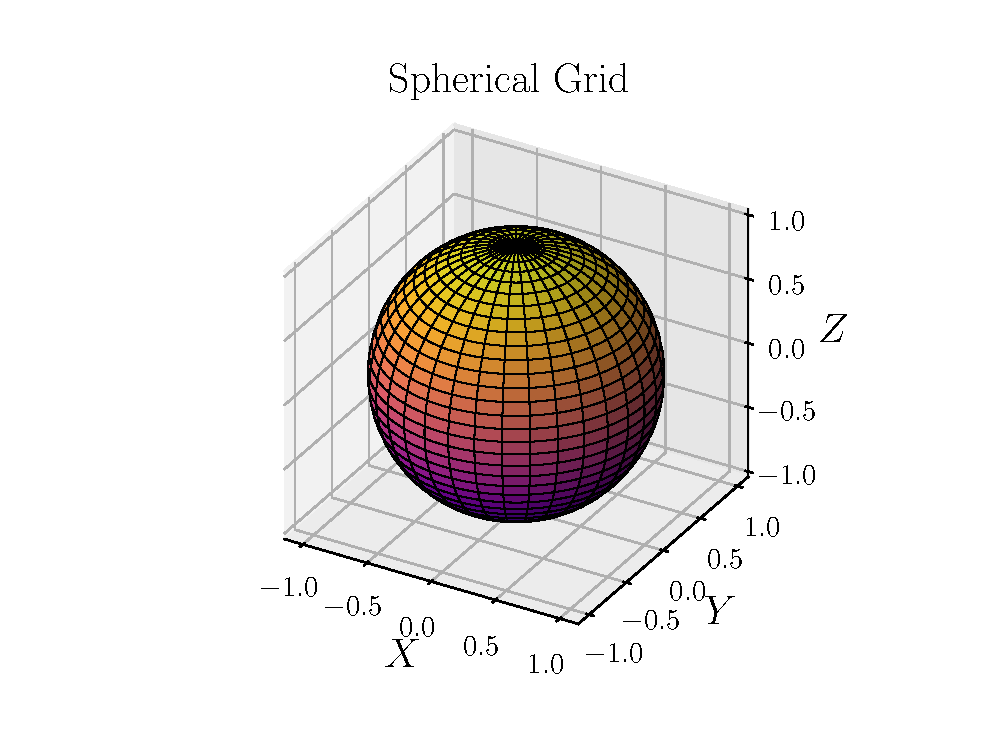
\includegraphics[width=0.4\textwidth]{img/Spherical_Grid.eps}

          }
          \subfloat[取其中一个四棱锥]
          {
              \label{fig:subfig2}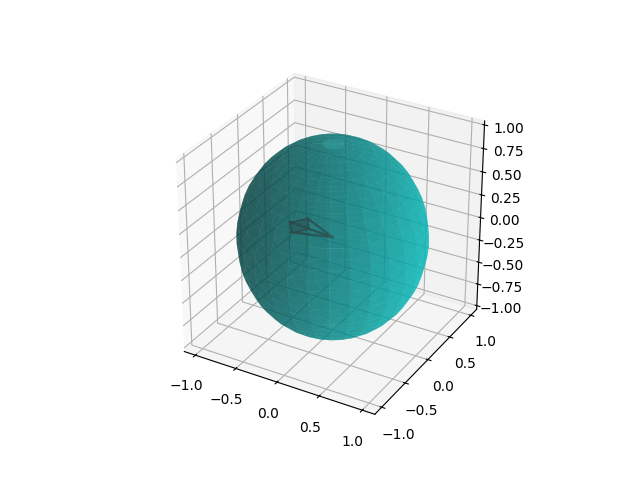
\includegraphics[width=0.4\textwidth]{img/GetOne.png}
          }
          \caption{球体公式推导}    % 整个图片的说明, 注释写在{}内
          \label{fig:subfig_1}            % 整个图片的标签编号, 注意这里跟子图是一样的道理, 标签不能重复 
        \end{figure}

        当n越大, 每个小网格越小时, 每个``小锥体"的底面就越平, ``小锥体"就越近似于棱锥, 其高越近似于球半径$R$. 设$O-ABCD$是其中一个``小锥体", 它的体积是:
        $$
        V_{O-ABCD}\approx \frac{1}{3}S_{ABCD}R
        $$
        由于球的体积就是这7个``小锥体"的体积之和, 而这7个``小锥体"的底面积之和就是球的表面积. 因此球(Spherical)的体积:
        $$
        V_{Spherical} = \frac{1}{3}S_{Spherical}R=\frac{1}{3}\times 4\pi R^2\cdot R=\frac{4}{3}\pi R^3
        $$
        \section{\textcolor[rgb]{0.11,0.65,0.52}{P121}}
        \textcolor[rgb]{0.38,0.11,0.2}{祖暅原理}: 夹在两个平行平面之间的两个几何体, 被平行于这两个平面的任意平面所截的两个截面的面积总相等, 那么两个几何体的体积相等.

        \begin{figure}[htbp]
            \centering
            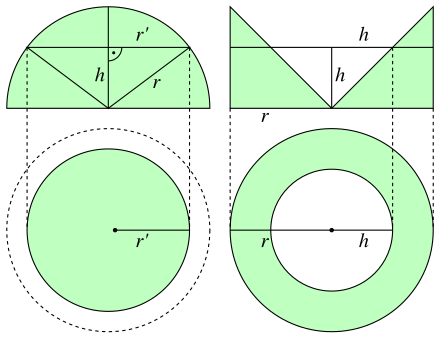
\includegraphics[width=0.5\textwidth]{img/Cavalieri_half-ball.svg.png}
            \caption{圆柱内切球体}
        \end{figure}

        如图8所示: 从其中一层以垂直表面的高$h$横切半径为$r$的半球体, 根据勾股定理, 半径为${\displaystyle r'={\sqrt {r^{2}-h^{2}}}}$, 所以横切面积是$${\displaystyle \pi \cdot (r')^{2}=\pi \cdot (r^{2}-h^{2})}$$对照立体是个有与半球体相同横切面积和高的立体, 中间有一圆锥体. 高$h$的对照立体环形切面有内圆周$h$及外圆周$r$, 其面积为$${\displaystyle \pi \cdot r^{2}-\pi \cdot h^{2}=\pi \cdot (r^{2}-h^{2})}$$因此两个立体都满足祖暅原理并有相同体积. 对照立体的体积就是圆柱体和圆锥体体积之差, 所以$${\displaystyle \pi \cdot r^{2}\cdot r-{\frac {1}{3}}\cdot \pi \cdot r^{2}\cdot r={\frac {2}{3}}\pi \cdot r^{3}}$$成功利用这条有名的方程计出半球体积, 从而导出球体积公式. 

        \chapter{选择性必修一}
        \section{\textcolor[rgb]{0.11,0.65,0.52}{P10, T8}}
        \begin{boxB}
            用向量方法证明: 在平面内的一条直线, 如果与这个平面的一条斜线在这个平面上的射影垂直, 那么它也与这条斜线垂直.
        \end{boxB}
        本题实际上是证明\textcolor[rgb]{0.38,0.11,0.2}{三垂线定理}.

        
        \begin{figure}[htbp]
            \centering
            \tdplotsetmaincoords{70}{110}
        \begin{tikzpicture}[yscale=2,xscale=2,line width=0.8pt,tdplot_main_coords]
            %% ===========================================
            \coordinate (A) at (0,0,0);
            \coordinate (B) at (4,0,0);
            \coordinate (C) at (4,3,0);
            \coordinate (D) at (0,3,0);
            
            \coordinate (A1) at (2,1,0);
            \coordinate (B1) at (2,1,2);
            \coordinate (O) at (2,2,0);
            \coordinate (C1) at (1,2,0);
            \coordinate (D1) at (3,2,0);
            % %% ===========================================
            % \draw[rounded corners=0.05pt](D1)circle (0.25pt)node[right]{$D_1$}--(A1)circle (0.25pt)node[above]{$A_1$}--(B1)circle (0.25pt)node[left=2pt]{$B_1$}--
            % (C1)circle (0.25pt)node[above=2pt]{$C_1$}--(D1)--(D)circle (0.25pt)node[right=2pt]{$D$}(C)circle (0.25pt)node[below=2pt]{$C$}--
            % (B)circle (0.25pt)node[below=2pt]{$B$}--(M)circle (0.25pt)node[left=2pt]{$M$}
            % (B1)--(C1)--(C)--(M)--(B1)(C)--(D)(A)circle (0.25pt)node[left=4pt,above]{$A$};
            % %% ===========================================
            % \draw[thin,dash pattern=on 3pt off 2pt](A1)--(A)
            % (B)--(A)--(D)(A)--(A1)--(M)--(A1)--(C);

            %% ===========================================
            \draw[rounded corners=0.05pt](A)--(B)circle (0.25pt)node[above=2.5pt,right=3pt]{$\alpha$}--(C)--(D)--(A);
            \draw[rounded corners=0.05pt](A1)circle (0.25pt)node[above=2.5pt,left=3pt]{$A$}--(B1)circle (0.25pt)node[above=2.5pt,right=3pt]{$B$}--(O)circle (0.25pt)node[above=1pt,right=1pt]{$O$}--(A1);
            \draw[rounded corners=0.05pt](D1)circle (0.25pt)node[above=2.5pt,left=3pt]{$D$}--(C1)circle (0.25pt)node[above=2.5pt]{$C$};
        \end{tikzpicture}
            \caption{三垂线定理}
        \end{figure}
        如图9所示: $BO \bot $平面$\alpha$, $CD\bot AO$, 因为$BA \bot $平面$\alpha$, $CD\subset $平面$\alpha$, 所以$$BA\bot CD\Longrightarrow \overrightarrow{BA}\cdot \overrightarrow{CD}=0$$.
        又有$CD\bot AO$, 所以$\overrightarrow{CD}\cdot \overrightarrow{AO}=0$.
        又因为$\overrightarrow{BO}=\overrightarrow{BA}+\overrightarrow{AO}$, 可得$$\overrightarrow{CD}\cdot\overrightarrow{BO}=\overrightarrow{CD}\cdot\left( \overrightarrow{BA}+\overrightarrow{AO} \right)$$
        展开括号表达式可得$$\overrightarrow{CD}\cdot\overrightarrow{BA}+\overrightarrow{CD}\cdot\overrightarrow{AO}=0. \blacksquare$$
        可以通过此方法配合几何知识来处理二面角的问题.
        \section{\textcolor[rgb]{0.11,0.65,0.52}{P68, P89, T10}}
        \begin{figure}[htbp]
            \centering
            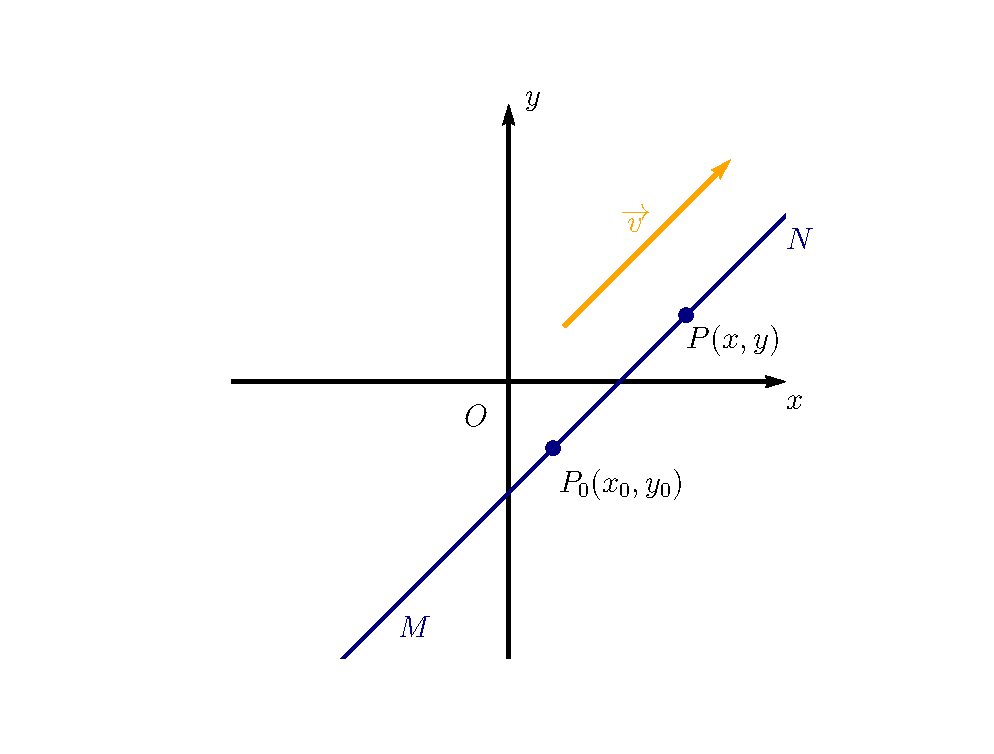
\includegraphics[width=0.7\textwidth]{img/ArgumentFunctions.eps}
            \caption{直线的参数方程}
        \end{figure}
        \textcolor[rgb]{0.38,0.11,0.2}{直线的参数方程}

        如图10所示: $\overrightarrow{v}=\left( m, n \right)$有$\overrightarrow{PP_0}=t\overrightarrow{v}\Longrightarrow  \left( x-x_0, y-y_0 \right)=t\left( m,n \right)$

        其中$(m,n)$的几何意义表示该直线的方向向量.

        \textcolor[rgb]{0.38,0.11,0.2}{圆的参数方程}

        已知圆的标准方程形如$$\displaystyle \left( x-a \right)^2+\left( y-b \right)^2=r^2$$
        将其转化为\textcolor[rgb]{0.75,0.17,0.22}{单位圆}$$\left( \frac{x-a}{r} \right)^2+\left( \frac{y-b}{r} \right)^2=1$$
        \textcolor[rgb]{0.75,0.17,0.22}{对比勾股定理}$\cos^2\theta +\sin^2\theta=1$有:
        $$\cos \theta =\frac{x-a}{r},\sin \theta=\frac{y-b}{r}$$
        解得:$$x=a+r\cos \theta,y=b+r\sin \theta, \blacksquare$$

        \section{\textcolor[rgb]{0.11,0.65,0.52}{P89, T9}}
        
        \begin{boxB}
            已知动点$M$与两个定点$O\left( 0,0 \right),A\left( 3,0 \right)$的距离之比为$\displaystyle \frac{1}{2}$, 求动点$M$的轨迹方程
        \end{boxB}

        本题实际上考察著名模型\textcolor[rgb]{0.38,0.11,0.2}{阿氏圆}的相关知识, 下面我们来解决这一道题目.

        设动点$M\left( x,y \right)$, 我们可以得到两条线的距离$$|MO|=\sqrt{x^2+y^2},|MA|=\sqrt{\left( x-3 \right)^2+y^2}$$
        所以$M$与两个定点的距离之比为$$d=\frac{\sqrt{x^2+y^2}}{\sqrt{\left( x-3 \right)^2+y^2}}=\frac{1}{2}$$
        将其化简可得$$\left( x+1 \right)^2+y^2=4$$
        \begin{figure}[htbp]
            \centering
            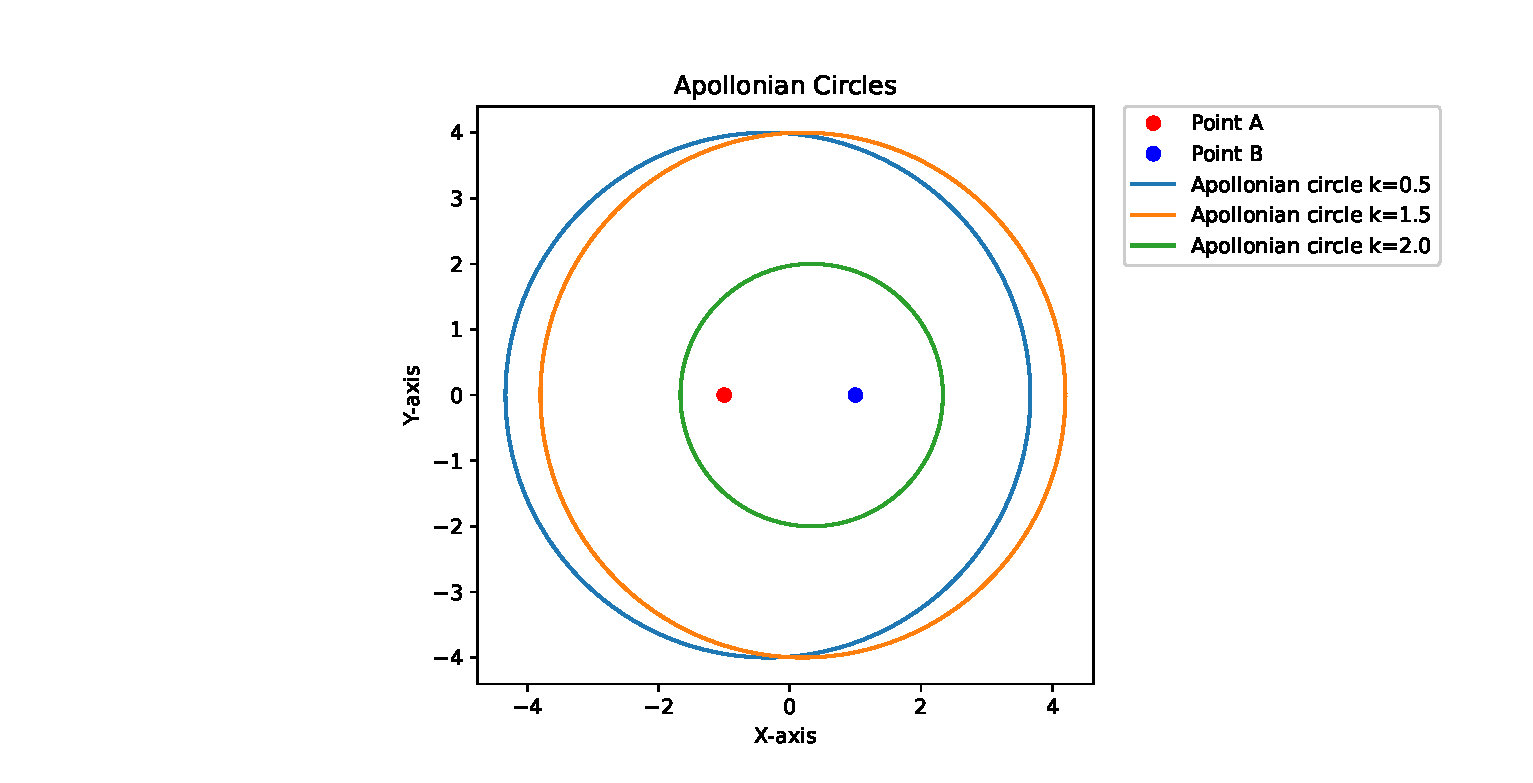
\includegraphics[width=\textwidth]{img/ApollonianCircles.eps}
            \caption{阿波罗尼斯圆}
        \end{figure}

        相关拓展知识:

        \begin{enumerate}
            \item 到两定点的距离之商为定值$(\neq 1)$的点的轨迹是阿氏圆
            \item 如图11所示: 若$P$到两定点$A$,$B$的距离之商为定值$k(k>0,k\neq1)$若$AB=a$,则其半径为$\displaystyle r=\frac{ac}{\left| k^2-1 \right|}$
            \item 如果$A,B$关于原点对称, 其中$A(-a,0)B(a,0)$且距离之商为定值$k(k>0,k\neq 1)$则圆心坐标为$\displaystyle \left( \frac{a\left( k^2+1 \right)}{k^2-1},0 \right)$, 半径$\displaystyle r=\frac{2ak}{\left| k^2-1 \right|}$
        \end{enumerate}
        \section{\textcolor[rgb]{0.11,0.65,0.52}{P89, T15}}
        此处提及\textcolor[rgb]{0.38,0.11,0.2}{切线方程}和\textcolor[rgb]{0.38,0.11,0.2}{切点弦方程}
        \begin{boxB}
            设圆$\displaystyle O:\left( x-a \right)^2+\left( y-b \right)^2=r^2$, 一条直线与圆相切于点$P\left( x_0,y_0 \right)$, 求切线方程.
        \end{boxB}

        已知\textcolor[rgb]{0.75,0.17,0.22}{切线斜率与$OP$垂直}, 故有$$
        k\cdot \frac{y_0-b}{x_0-a}-1\Longrightarrow k=-\frac{x_0-a}{y_0-b}
        $$
        利用点斜式可写出$$y-y_0=-\frac{x_0-a}{y_0-b}\left( x-x_0 \right)$$
        整理可得到直线方程$$\left( x_0-a \right)\left( x-a \right)+\left( y_0-b \right)\left( y-b \right)=r^2.\blacksquare$$

        \begin{figure}[htbp]
            \centering
            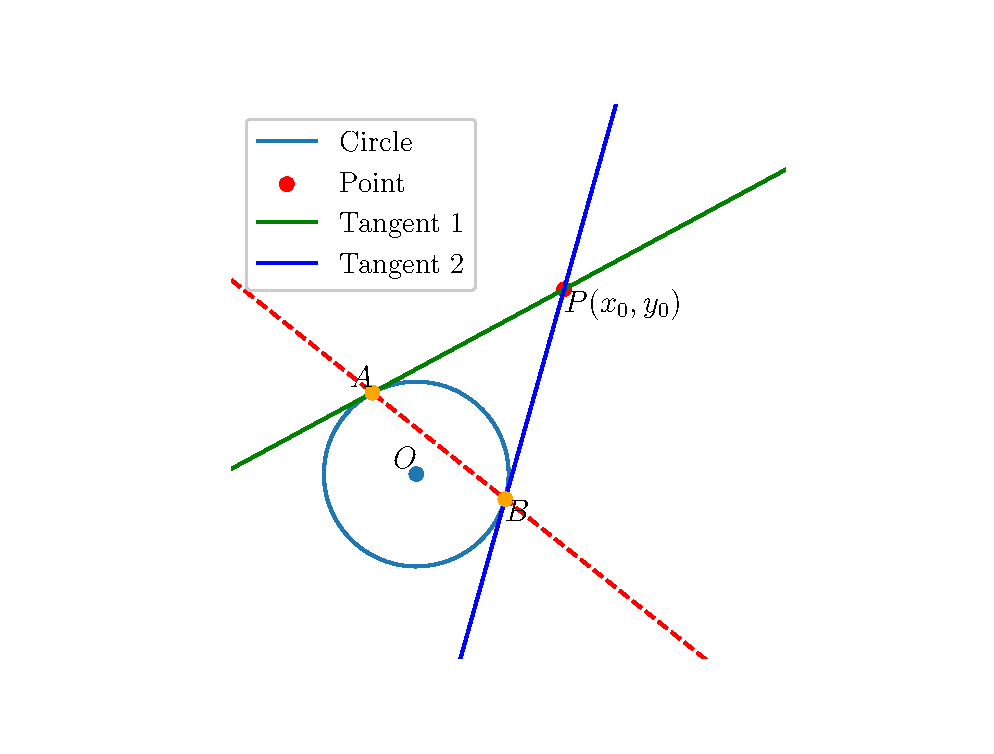
\includegraphics[width=0.8\textwidth]{img/TangentOfCircle.eps}
            \caption{切点弦}
        \end{figure}
        
        如图12所示: 如何求求切点弦方程$l_{AB}$?

        设$A(x_1,y_1)$, 则$$l_{AP}:\left( x_1-a \right)\left( x-a \right)+\left( y_1-b \right)\left( y-b \right)=r^2$$
        设$B(x_2,y_2)$, 则$$l_{BP}:\left( x_2-a \right)\left( x-a \right)+\left( y_2-b \right)\left( y-b \right)=r^2$$
        此时$A,B$两点均在$l_{AB}$的直线上, 所以利用\textcolor[rgb]{0.75,0.17,0.22}{同构}可得$$l_{AB}=\left( x_0-a \right)\left( x-a \right)+\left( y_0-b \right)\left( y-b \right)=r^2$$
        %% todo
        \section{\textcolor[rgb]{0.11,0.65,0.52}{P108, 例3; P126, T1}}
        \begin{boxB}
            设$A,B$两点分别为$(-a,0),(a,0)$,设$AM,BM$相交于点$M$,且它们斜率之积为$\displaystyle -\frac{b^2}{a^2}$, 求$M$的轨迹方程. 
        \end{boxB}

        \textcolor[rgb]{0.38,0.11,0.2}{圆锥曲线第三定义}

        设$M(x,y)$, 则$$k_{AM}=\frac{y}{x+a},k_{BM}=\frac{y}{x-a}\Longrightarrow k_{AM}k_{BM}=\frac{y^2}{x^2-a^2}=-\frac{b^2}{a^2}$$
        化简可得$$a^2y^2=-b^2x^2+a^2b^2\Longrightarrow \frac{a^2}{x^2}+\frac{b^2}{y^2}=1(\mathrm{Remove} (-a,0)(a,0))$$
        若改为斜率之积$\frac{b^2}{a^2}$, 其它不变, 则有$\displaystyle k_{AM}k_{BM}=\frac{y^2}{x^2-a^2}=\frac{b^2}{a^2}$即可得到$\displaystyle \frac{x^2}{a^2}-\frac{y^2}{b^2}=1$(其中$(-a,0)$与$(a,0)$除去), 由于椭圆$a^2=b^2+c^2$, 双曲线有$c^2=a^2+b^2$, 故可\textcolor[rgb]{0.75,0.17,0.22}{统一为$k_{AM}k_{BM}=e^2-1$}

        更一般的结论, 只要过原点的直线$l$与椭圆或双曲线相交$A,B$两点,$M$为曲线上任意一点, 都满足$k_{AM}k_{Bw}=e^2-1$成立.
        \section{\textcolor[rgb]{0.11,0.65,0.52}{P108, 思考}}
        此处实际上有涉及\textcolor[rgb]{0.38,0.11,0.2}{仿射变换}.
        
        椭圆方程$\displaystyle \frac{x^2}{a^2}+\frac{y^2}{b^2}=1$, 此时若\textcolor[rgb]{0.75,0.17,0.22}{把$x$轴缩放$a$倍记作$x'$, $y$轴缩放$b$倍记作$y'$}, 则有$\displaystyle x'=\frac{x}{a},y'=\frac{y}{b}\Longrightarrow x'^2+y'^2=1$.

        实际上是对整个坐标系进行一个线性变换, 将向量基底$\boldsymbol{e_1}=(1,0),\boldsymbol{e_2}=(0,1)$缩放为$\displaystyle \boldsymbol{e_1'}=(\frac{1}{a},0),\boldsymbol{e_2'}=(0,\frac{1}{b})$
        
        \begin{figure}[htbp]
            \centering
            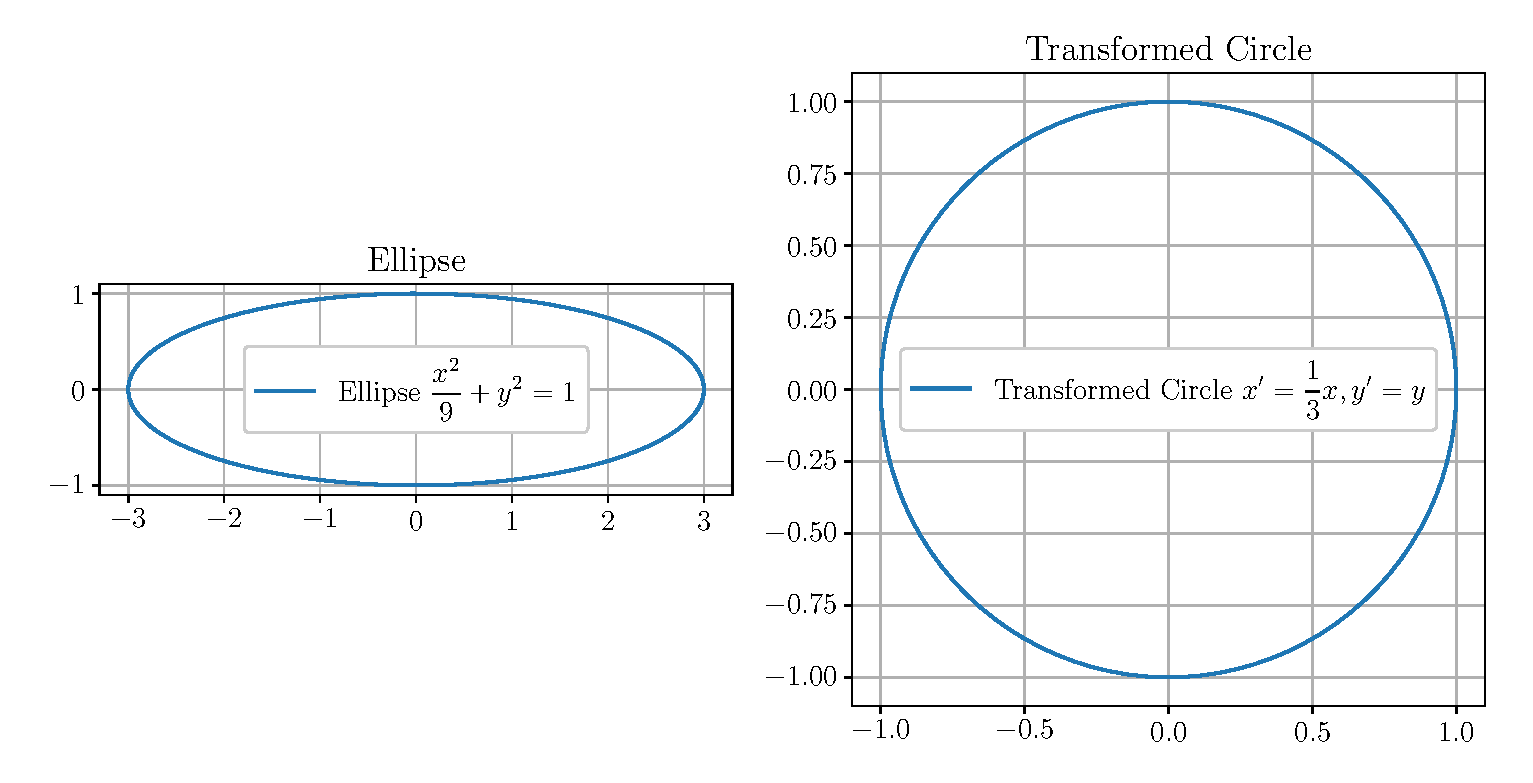
\includegraphics[width=\textwidth]{img/AffineTransform.eps}
            \caption{仿射变换}
        \end{figure}

        仿射变换的一些性质:
        \begin{enumerate}
            \item 两个共线向量变化前后均共线(相互平行的两条直线变化前后均平行);
            \item 仿射变换保持共线几点的分比;
            \item 变换后平面内任意一条直线的斜率变为原来的$\displaystyle \frac{a}{b}$, 面积变为原来的$\displaystyle \frac{1}{ab}$.
        \end{enumerate}

        大家可以试着用上面的仿射变换证明一下刚刚提及的圆曲第三定义, 需要注意的是, 这一个方法不能用于高考的简答题, 否则你可能会面临只得答案分的风险.

        \section{\textcolor[rgb]{0.11,0.65,0.52}{P108, 思考, 拓展}}

        这一部分感兴趣选读.

        上面讲到了椭圆的仿射, 那么同为圆锥曲线, 看上去标准方程结构差不多的双曲线是否可以做到类似的变换来将上面的每一个点映射到圆上呢?

        这就扯到一种复变换叫做 Möbius 变换, 对于复平面上的双曲线, 可以通过某些 Möbius 变换将其映射到单位圆. 这种变换的一般形式是:$$z'=\frac{az+b}{cz+d},ad-bc\neq 0$$
        
        在复平面$xOy$中, 任意一个复数可表示为$z=a+bi,a,b\in \mathbb{R}$的形式, 其中$(a,b)$为这个复平面上的点, 因此在复平面上圆的方程为:$$\left| z \right|=r$$

        有一复数$z_0=a_0+b_0i$在屏幕上的点位于圆上, 那么这个圆的切线方程为$$\mathrm{Re}\left( \bar{z_0}z \right)=r^2$$

        事实上如果将双曲线的 \( y \) 轴变为虚数数轴, 即将原来的实数 \( y \) 替换为纯虚数 \( iy \)(其中 \( i \) 是虚数单位, \( i^2 = -1 \)), 那么双曲线的标准方程会发生变化. 

        考虑标准的双曲线方程: 
        \[
        \frac{x^2}{a^2} - \frac{y^2}{b^2} = 1
        \]
        当将 \( y \) 变为虚数 \( iy \), 方程变为: 
        \[
        \frac{x^2}{a^2} - \frac{(iy)^2}{b^2} = 1
        \]
        
        由于 \( (iy)^2 = -y^2 \), 方程变为: 
        \[
        \frac{x^2}{a^2} + \frac{y^2}{b^2} = 1
        \]
        
        这个方程其实是一个椭圆的方程, 因此, 当将双曲线的 \( y \) 轴变为虚数轴时, 双曲线的方程变成了椭圆的方程.

        在复平面中, 复数 \( z = x + iy \) 由实部 \( x \) 和虚部 \( y \) 表示, 其中 \( x \) 和 \( y \) 分别代表复数的实数部分和虚数部分. 对于圆来说, 方程 \( |z| = r \) 描述的是到原点距离为 \( r \) 的点的集合, 也就是: 
        \[
        |z| = |x + iy| = \sqrt{x^2 + y^2} = r
        \]
        这是一个以原点为中心, 半径为 \( r \) 的圆. 

    现在我们来推导复平面上与双曲线相对应的方程. 双曲线的一个特征是两个焦点, 且对每个点, 其到两个焦点的距离之差的绝对值是一个常数. 在复平面中, 这意味着我们可以将双曲线用类似的距离关系来表示. 

    设复平面上有两个焦点 \( z_1 \) 和 \( z_2 \), 则双曲线可以定义为满足以下条件的点的集合: 
    \[
    |z - z_1| - |z - z_2| = \text{常数}
    \]
    或者为了简化讨论, 可以取绝对值后方程为: 
    \[
    ||z - z_1| - |z - z_2|| = 2a
    \]
    其中, \( 2a \) 是双曲线的实轴长度. 

    这个方程表示复平面上到两个焦点 \( z_1 \) 和 \( z_2 \) 的距离差的绝对值为常数的点的集合, 与实平面中双曲线的定义一致. 

    因此, 复平面上的双曲线可以表示为满足以下条件的点的集合: 
    \[
    |z - z_1| - |z - z_2| = \text{常数}
    \]
    这是复数形式下双曲线的标准表达方式. \cite{complex}

    感兴趣的同学可以使用复变换来解决双曲线问题, 但是请不要沉迷于技巧中.

    \section{\textcolor[rgb]{0.11,0.65,0.52}{P117, P127, T10}}

    这里是\textcolor[rgb]{0.38,0.11,0.2}{圆锥曲线的第二定义}:

    若点 $M(x,y)$ 与定点 $F(c,O)$ (或$F'(-c,0)$)的距离和它到直线$\displaystyle l:x=\frac{a^2}{c}$(或$\displaystyle l':x=\frac{a^2}{c}$)的距离的比是常数$\displaystyle \frac{c}{a}(0<c<a)$则点M的轨迹是一个椭圆(如图14), 这是从另一个角度给出了椭圆的定义.

    \begin{figure}[htbp]
        \centering
        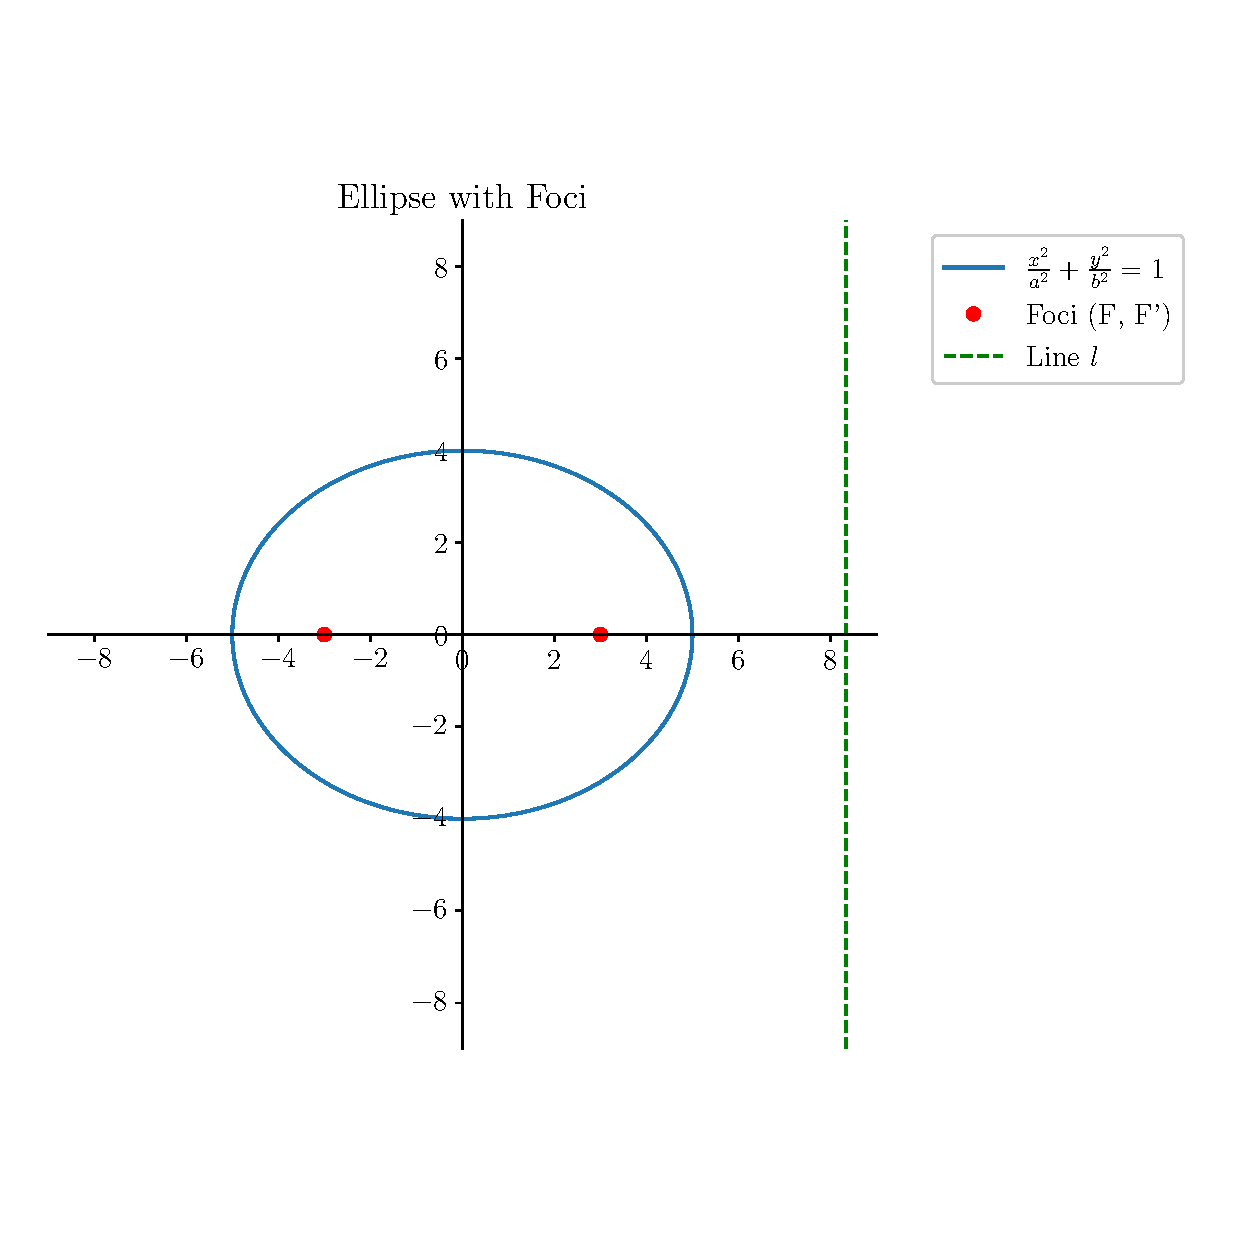
\includegraphics[width=0.8\textwidth]{img/ConicSection2Define.eps}
        \caption{椭圆的第二定义}
    \end{figure}

    这里定点$F(c,O)$是椭圆的一个焦点,直线$\displaystyle l:x=\frac{a^2}{c}$称为相应于焦点F的准线.

    在推导椭圆标准方程时, 我们曾得到
    \begin{equation}
        a^2-cx=a\sqrt{(x-c)^2+y^2}
    \end{equation}
    如果把(3)式变形为
    \begin{equation}
        \frac{\sqrt{\left( x-c \right)^2+y^2}}{\displaystyle \frac{a^2}{c}-x}=\frac{c}{a}
    \end{equation}
    则(4)式的几何意义就是动点$M(x,y)$与定点$F(c,O)$的距离和动点$M$到定直线$\displaystyle l:x=\frac{a^2}{c}$的距离的比是常数$\displaystyle \frac{c}{a}$

    双曲线其它条件也是一样的, 只是$c>a$.

    \section{\textcolor[rgb]{0.11,0.65,0.52}{P134 $\sim$ P139}}

    这里涉及抛物线\textcolor[rgb]{0.38,0.11,0.2}{焦半径, 焦点弦}诸多结论.

    设$P\left( x_0,y_0 \right)$是抛物线$y^2=2px$上一点, $\displaystyle \left| PF \right|=\left| PT \right|=\left| PQ \right|+\left| QT \right|=x_0+\frac{p}{2}$
    \begin{figure}[htbp]
        \centering
        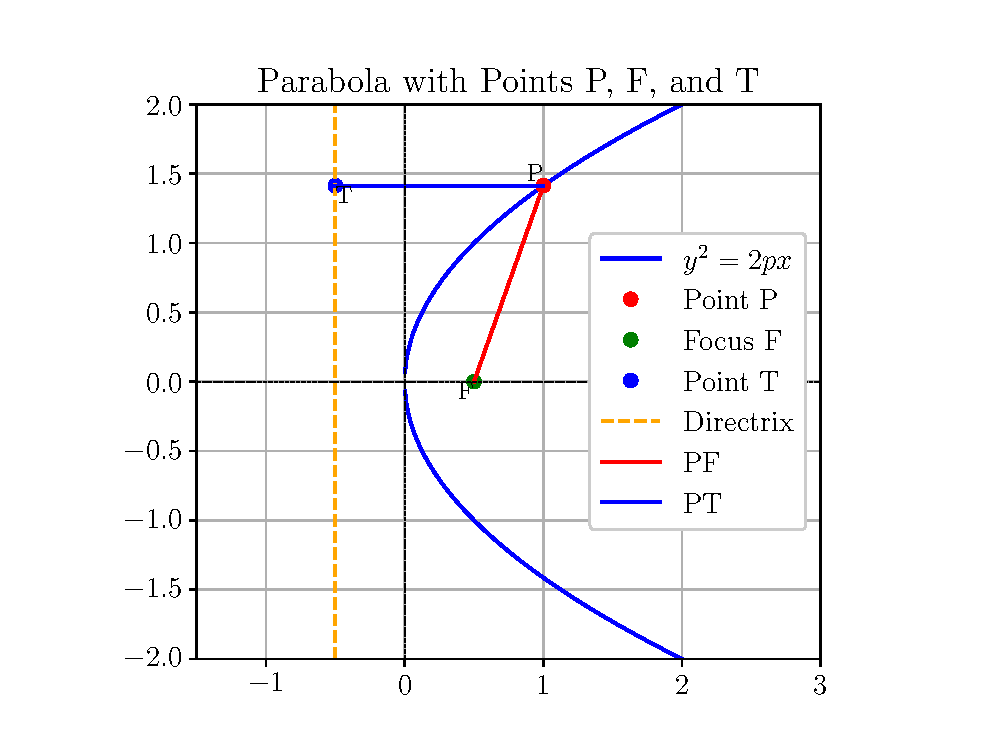
\includegraphics[width=0.8\textwidth]{img/ParabolaFocusRadius.eps}
        \caption{抛物线焦半径}
    \end{figure}

    设$A(x_1,y_1),B(x_2,y_2),\angle AFx=\theta$, 抛物线$y^2=2px$有:

    \begin{enumerate}
        \item $$\left| AB \right|=x_1+x_2+p=\frac{2p}{\sin^2\theta}$$
        \item $$\left| AF \right|=\frac{p}{1-\cos \theta};\left| BF \right|=\frac{p}{1+\cos \theta}$$
        \item $$\frac{1}{\left| AF \right|}+\frac{1}{\left| BF \right|}=\frac{2}{p}$$
        \item 若$\displaystyle \frac{\left| AF \right|}{\left| BF \right|}=x>0$则$\displaystyle \cos \theta = \frac{x-1}{x+1}$
        \item $\displaystyle x_1x_2=\frac{p^2}{4},y_1y_2=p^2$
        \item \dots\dots
    \end{enumerate}

    \section{\textcolor[rgb]{0.11,0.65,0.52}{P140}}

    圆锥曲线的光学性质及其应用.

    椭圆、双曲线、拋物线这些圆锥曲线都有焦点, 焦点, 顾名思义, 就是光线的聚築点. 这说明圆锥曲线与光线有紧密的联系, 圆锥曲线具有丰富的光学性质.

    我们知道, 当一来光线照到镜而时, 光线会依一定的规律反射, 即反射角等于入射角.当光照射到曲面时, 特别是由圆锥曲线绕共对称轴旋转而成的曲面时, 会有什么现象呢?

    我们看生活中的一个实例:一只很小的灯泡发出的光, 会分散地射向各方, 但把它装在圆柱形手电简里, 经过适当调节, 就能射出一来比较强的干行光线, 这是为什么呢?

    \begin{figure}[htbp]
        \centering
        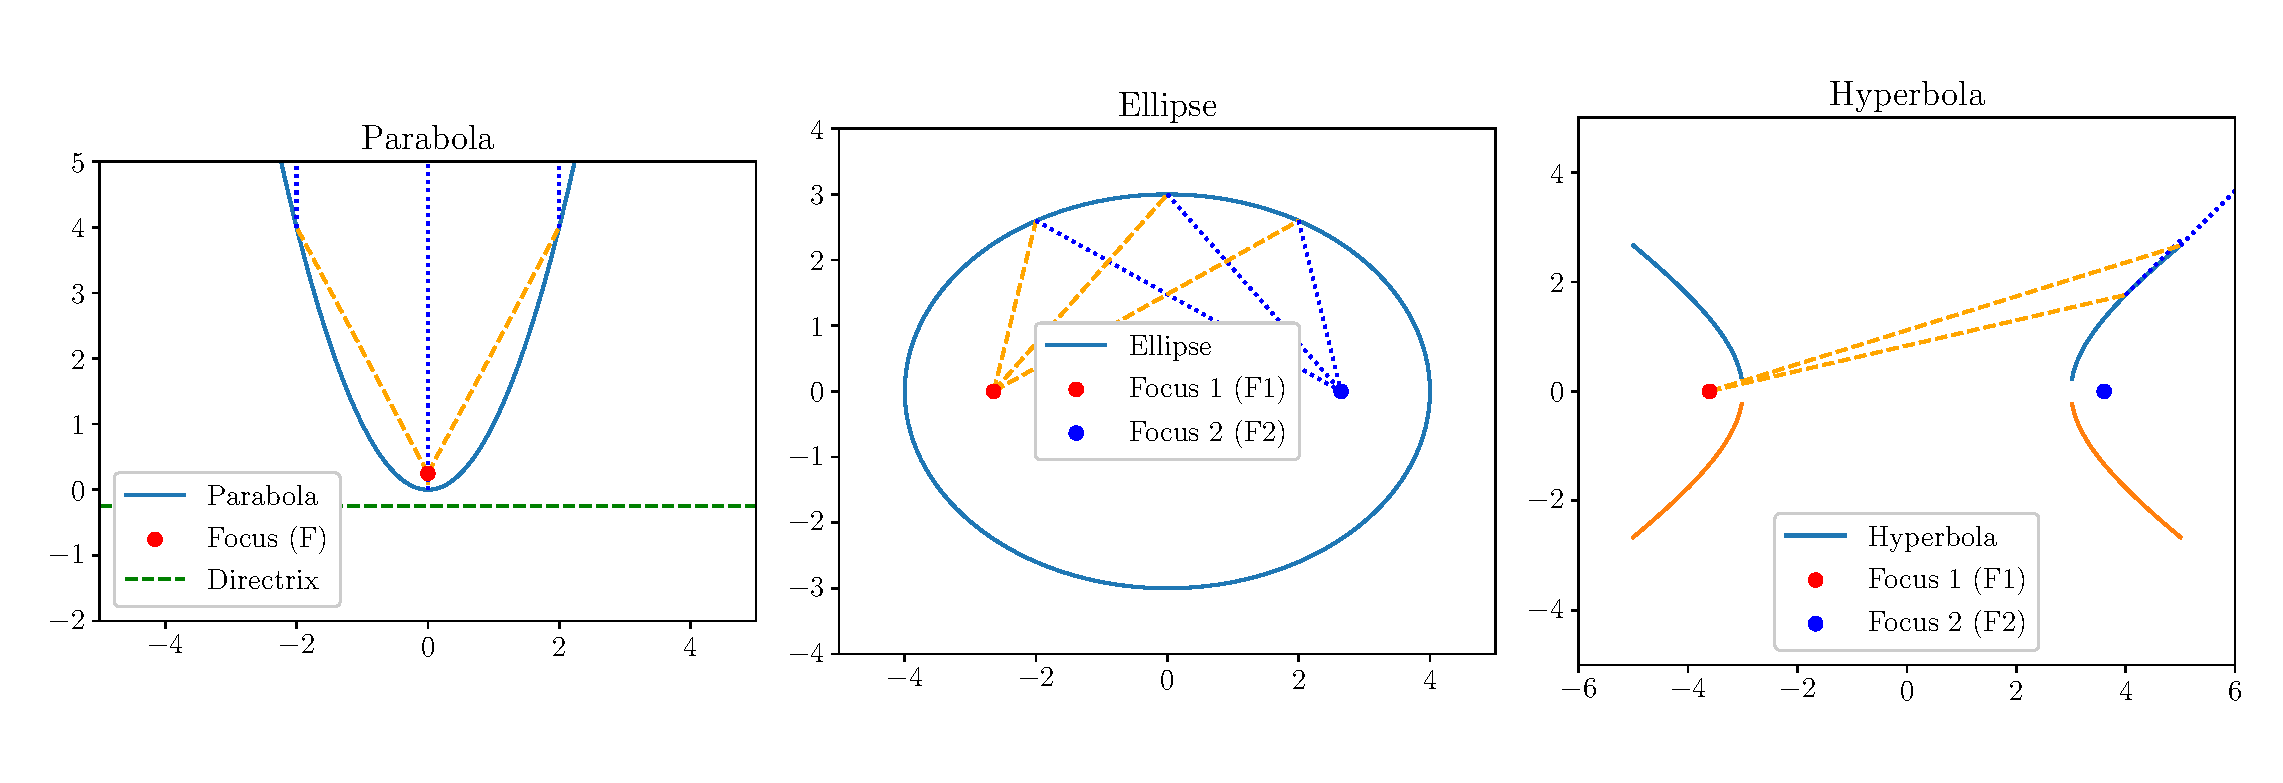
\includegraphics[width=\textwidth]{img/ConicCurveLightAttribute.eps}
        \caption{圆锥曲线光学性质}
    \end{figure}

    原来手电筒内, 在小灯泡后而有一个反光镜, 镜而的形状是一个由抛物线绕它的对称轴旋转所得到的曲面, 这种曲面叫做抛物而.拋物线有一条重要性质:从焦点发出的光线, 经过抛物线上的一点反射后, 反射光线平行于抛物线的轴, 探照灯也是利用这个原理设计的.

    应用抛物线的这个性质, 也可以使一来平行于抛物线的轴的光线, 经过拋物面的反射集中于它的焦点.人们应用这个原理, 设计了一种加热水和食物的太阳灶.在这种太阳灶上装有一个旋转抛物面形的反光镜, 当它的轴与太阳光线平行时, 太阳光线经过反射后集中于焦点处, 这一点的溫度就会很高.

    椭圆和双曲线的光学性质与抛物线不同. 从椭圆的一个焦点发出的光线, 经过椭圆反射后, 反射光线交于椭圆的另一个焦点上从双曲线的一个焦点发出的光线, 经过双曲线反射后, 反射光线是散开的, 它们就好像是从另一个焦点射出的一样. 椭圆、双曲线的光学性质也被人们广泛地应用于各种设计中.

    \chapter{选择性必修二}
    
    \section{\textcolor[rgb]{0.11,0.65,0.52}{P10, P57 T17}}
    \subsection{斐波那契数列引论}
    \textcolor[rgb]{0.38,0.11,0.2}{斐波那契数列}递推公式:$$a_{n+2}=a_n+a_{n+1},a_1=a_2=1$$

    下面是该数列的性质:

    \begin{enumerate}
        \item 当$n$为奇数的时候, $a_1+a_3+a_5+\cdots+a_n=a_2+a_3+a_5+\cdots+a_n$, 又因为$a_{n+2}=a_n+a_{n+1}$故原式$=a_4+a_5+a_7+\cdots+a_n=a_{n+1}$;
        \item 当$n$为偶数的时候, $a_2+a_4+a_6+\cdots+a_n=a_1+a_2+a_4+a_6+\cdots+a_n-1$(多配凑a1), 原式等于$a_3+a_4+a_6+\cdots+a_n-1=a_{n+1}-1$
        \item $\displaystyle a_1^2+a_2^2+a_3^2+\cdots+a_n^2=a_na_{n+1}$
    \end{enumerate}

    接下来我们来证明第三个结论:
    $$a_{n+2}=a_{n+1}=a_n\Longrightarrow a_{n+1}=a_{n+2}-a_n$$
    等式两边同乘$a_{n+1}$:$$a_{n+1}^2=a_{n+1}\left( a_{n+2}-a_n \right)=a_{n+1}a_{n+2}-a_{n+1}a_n$$
    又有:$$\left\{\begin{matrix} 
        a_2^2=a_3a_2-a_2a_1 \\  
        a_3^2=a_4a_3-a_3a_2 \\
        a_4^2=a_5a_4-a_4a_3 \\
        \cdots \\
        a_n^2=a_{n+1}a_n-a_{n}a_{n-1}
      \end{matrix}\right. $$
    累加可得$$a_2^2+a_3^2+a_4^2+\cdots+a_n^2=a_3a_2-a_2a_1+a_4a_3-a_3a_2+\cdots+a_{n+1}a_n-a_{n}a_{n-1}$$
    最后化简可得$$a_2^2+a_3^2+a_4^2+\cdots+a_n^2=a_na_{n+1}-a_1a_2,a_1a_2=a_1^2$$
    移项可得$\displaystyle a_1^2+a_2^2+a_3^2+\cdots+a_n^2=a_na_{n+1}. \blacksquare$

    \subsection{递推公式的推导}
    下面拓展斐波那契数列的递推公式的推导:

    构建等比数列$${\displaystyle a_{n}+\alpha a_{n-1}=\beta (a_{n-1}+\alpha a_{n-2})}$$
    化简得到$${\displaystyle a_{n}=(\beta -\alpha )a_{n-1}+\alpha \beta a_{n-2}}$$
    比较系数可得:$${\displaystyle {\begin{cases}\beta -\alpha =1\\\alpha \beta =1\end{cases}}}$$
    不妨设${\displaystyle \beta >0,\alpha >0}$, 将方程解出可得$${\displaystyle {\begin{cases}\alpha ={\dfrac {{\sqrt {5}}-1}{2}}\\\beta ={\dfrac {{\sqrt {5}}+1}{2}}\end{cases}}}$$
    又因为有${\displaystyle a_{n}+\alpha a_{n-1}=\beta (a_{n-1}+\alpha a_{n-2})}$, 即${\displaystyle \left\{a_{n}+\alpha a_{n-1}\right\}}$为等比数列.
    由以上可得:$${\displaystyle {\begin{aligned}a_{n+1}+\alpha a_{n}&=(a_{2}+\alpha a_{1})\beta ^{n-1}\\&=(1+\alpha )\beta ^{n-1}\\&=\beta ^{n}\\\end{aligned}}}$$
    将其变形可得$${\displaystyle {\frac {a_{n+1}}{\beta ^{n+1}}}+{\frac {\alpha }{\beta }}\cdot {\frac {a_{n}}{\beta ^{n}}}={\frac {1}{\beta }}}$$
    若令${\displaystyle b_{n}={\frac {a_{n}}{\beta ^{n}}}}$, 可得$${\displaystyle b_{n+1}+{\frac {\alpha }{\beta }}b_{n}={\frac {1}{\beta }}}$$
    设${\displaystyle b_{n+1}+\lambda =-{\frac {\alpha }{\beta }}(b_{n}+\lambda )}$解得${\displaystyle \lambda =-{\frac {1}{\alpha +\beta }}}$, 故数列${\displaystyle \left\{b_{n}+\lambda \right\}}$为等比数列, 即$${\displaystyle b_{n}+\lambda =\left(-{\frac {\alpha }{\beta }}\right)^{n-1}\left(b_{1}+\lambda \right)}$$
    而${\displaystyle b_{1}={\frac {a_{1}}{\beta }}={\frac {1}{\beta }}}$, 故有$${\displaystyle b_{n}+\lambda =\left(-{\frac {\alpha }{\beta }}\right)^{n-1}\left({\frac {1}{\beta }}+\lambda \right)}$$
    根据$\alpha$与$\beta$的值如下 $${\displaystyle {\begin{cases}\alpha ={\dfrac {{\sqrt {5}}-1}{2}}\\\beta ={\dfrac {{\sqrt {5}}+1}{2}}\end{cases}}} $$
    与${\displaystyle b_{n}={\frac {a_{n}}{\beta ^{n}}}}$可得$${\displaystyle a_{n}={\frac {\sqrt {5}}{5}}\cdot \left[\left({\frac {1+{\sqrt {5}}}{2}}\right)^{n}-\left({\frac {1-{\sqrt {5}}}{2}}\right)^{n}\right]}$$得出$    {\displaystyle {a_{n}}}$表达式$${\displaystyle a_{n}={\frac {\sqrt {5}}{5}}\cdot \left[\left({\frac {1+{\sqrt {5}}}{2}}\right)^{n}-\left({\frac {1-{\sqrt {5}}}{2}}\right)^{n}\right]}.\blacksquare$$ \cite{Fibonacci}
    \subsection{使用数学归纳法证明通项公式}
    证明${\displaystyle F_{n}={\frac {\sqrt {5}}{5}}\cdot \left[\left({\frac {1+{\sqrt {5}}}{2}}\right)^{n}-\left({\frac {1-{\sqrt {5}}}{2}}\right)^{n}\right]}$.

    设$\varphi={\displaystyle {\frac {1+{\sqrt {5}}}{2}}}$,当${\displaystyle n=1}$时$${\displaystyle {\frac {1}{\sqrt {5}}}[\varphi ^{1}-(1-\varphi )^{1}]={\frac {1}{\sqrt {5}}}[\varphi -1+\varphi ]={\frac {1}{\sqrt {5}}}[2\varphi -1]={\frac {1}{\sqrt {5}}}\times {\sqrt {5}}=1=F_{1}}$$
    设当${\displaystyle n=k}$及${\displaystyle n=k+1}$时皆成立, 即$${\displaystyle F_{k}={\frac {1}{\sqrt {5}}}[\varphi ^{k}-(1-\varphi )^{k}]},{\displaystyle F_{k+1}={\frac {1}{\sqrt {5}}}[\varphi ^{k+1}-(1-\varphi )^{k+1}]}$$
    因此, 根据数学归纳法原理, 此表达式对于任意正整数${\displaystyle n}$皆成立.$\blacksquare$ \cite{induction}

    \section{\textcolor[rgb]{0.11,0.65,0.52}{P47}}
    \begin{boxB}
        证明$\displaystyle 1^2+2^2+3^2+\cdots+n^2=\frac{n\left( n+1 \right)\left( 2n+1 \right)}{6}$
    \end{boxB}
    \subsection{数学归纳法}
    假设条件成立, 对通项进行归纳有
    \begin{equation}
        1^2+2^2+3^2+\cdots+n^2=\frac{n\left( n+1 \right)\left( 2n+1 \right)}{6}
    \end{equation}
    扩展到$n+1$项有
    \begin{equation}
        1^2+2^2+3^2+\cdots+n^2+\left( n+1 \right)^2=\frac{\left( n+1 \right)\left( n+2 \right)\left( 2n+3 \right)}{6}
    \end{equation}
    用(6)-(5)可得等式左边为$\left( n+1 \right)^2$, 等式右边化简得到$$\frac{\left( n+1 \right)\left( n+2 \right)\left( 2n+3 \right)}{6}-\frac{n\left( n+1 \right)\left( 2n+1 \right)}{6}=n^2+2n+1.\blacksquare$$
    \begin{boxB}
        小练习: 使用数学归纳法证明$$1^3+2^3+3^3+\cdots+n^3=\left( 1+2+3+\cdots+n \right)^2$$
    \end{boxB}
    \subsection{立方差裂项}
    利用立方差公式$$n^3-\left( n-1 \right)^3=3n^2-3n-1$$化简变形得$$n^2=\frac{1}{3}\left[ 3n-1+n^3-\left( n-1 \right)^3 \right]$$全部相加求和可得$$1^2+2^2+3^2+\cdots+n^2=\frac{1}{3}\left[ \frac{3n^2+n}{2}+n^3 \right]=\frac{2n^3+3n^2+n}{6}$$
    整理可得$$\sum_{i=1}^{n}\left ( i^2 \right )  =\frac{n(n+1)(2n+1)}{6} .\blacksquare$$

    总结操作: 此方法用到多项式的\textcolor[rgb]{0.75,0.17,0.22}{差分}操作, 利用$n^3-(n-1)^3$求和过程可约分来构造立方差公式的操作技巧.
    \section{\textcolor[rgb]{0.11,0.65,0.52}{P50}}
    \begin{boxB}
        证明: 若$x>-1,a>1$, 则$\displaystyle \left( 1+x \right)^a\ge 1+ax$; 若$x>-1,0<a<1$, 则$\displaystyle \left( 1+x \right)^a\le 1+ax$
    \end{boxB}
    此处涉及了\textcolor[rgb]{0.38,0.11,0.2}{伯努利不等式}下面是证明过程:

    此处证明第二种情况, 可自行类比第一种情况; 证明: $x>-1,0<a<1$, \textcolor[rgb]{0.75,0.17,0.22}{作差构造函数}, 令$\displaystyle f(x)=\left( 1+x \right)^a-1-ax$, 对其求导可得$$f'(x)=a\left[ \left( 1+x \right)^{a-1}-1 \right]$$
    当 $-1<x<0$ 时:$f'(x)>0$, $f(x)$单调递增, 当$x>0$时, $f'(x)<0$, $f(x)$单调递减.
    $$f(x)_{\max }=f(0)=0\Longrightarrow \left( 1+x \right)^a-1-ax\le 0\Longrightarrow \left( 1+x \right)^a\le 1+ax.\blacksquare$$

    \section{\textcolor[rgb]{0.11,0.65,0.52}{P52, T10}}

    本题涉及\textcolor[rgb]{0.38,0.11,0.2}{角谷猜想}.

    任取一个正整数, 若是奇数, 就将该数乘3再加上1, 若是偶数, 就将该数除以2, 反复进行上述两种运算, 经过有限次步骤后, 必入循环$1\rightarrow 4\rightarrow 2\rightarrow 1$这就是数学史上著名的``冰雹猜想"(角谷猜想)如取正整数$m=6$, 根据上述运算法则得出$6\rightarrow 3\rightarrow 10\rightarrow 5\rightarrow 16\rightarrow 8\rightarrow 4\rightarrow 2\rightarrow 1$, 共需8个步骤变为1(简称为8步``雹程"). 现给出递推关系如下
    
    已知数列$\left\{ a_n \right\}$满足$a_1=m,m\in \mathbb{Z}^+$,$\displaystyle a_{n+1}=\left\{\begin{matrix} 
        \displaystyle \frac{a_n}{2},a_n\in\left \{ x|x=2k,k\in \mathbb{Z}  \right \}    \\  
        3a_n+1 a_n\in\left \{ x|x=2k-1,k\in \mathbb{Z}  \right \}
      \end{matrix}\right. $
    
    (1)当$m=17$, 试确定$a_n=1$需要多少步雹程;

    (2)若$a_8=1$, 求$m$所有可能的取值集合.

    \vspace{2em}

    (1)17,52,26,13,40,20,10,5,16,8,4,2,1

    (2)从后往前倒推:$$1\rightarrow 2\rightarrow 4\rightarrow 8\rightarrow 16\rightarrow \left\{\begin{matrix} 
        32\rightarrow 64\rightarrow  \left\{\begin{matrix} 
        128\rightarrow 256\\  
        21\rightarrow 42
      \end{matrix}\right. \\  
        5\rightarrow 10\rightarrow \left\{\begin{matrix} 
        3\rightarrow 6\\  
        2\rightarrow 40
      \end{matrix}\right. \\  
      \end{matrix}\right. $$
    因此$m$的可能集合$m=\left\{ 6,40,42,256 \right\}$

    \section{\textcolor[rgb]{0.11,0.65,0.52}{P65}}
    教材在此处提及导数的定义($:=$符号表示右侧的式子记作左侧的符号)$$f'(x):=\lim_{\Delta x \to 0} \frac{f(x+\Delta x)-f(x)}{\Delta x} $$
    我们可以利用这个定义来证明圆的周长公式$C=2\pi r$为其面积公式$S=\pi r^2$对$r$的导数.

    \begin{figure}[htbp]
        \centering
        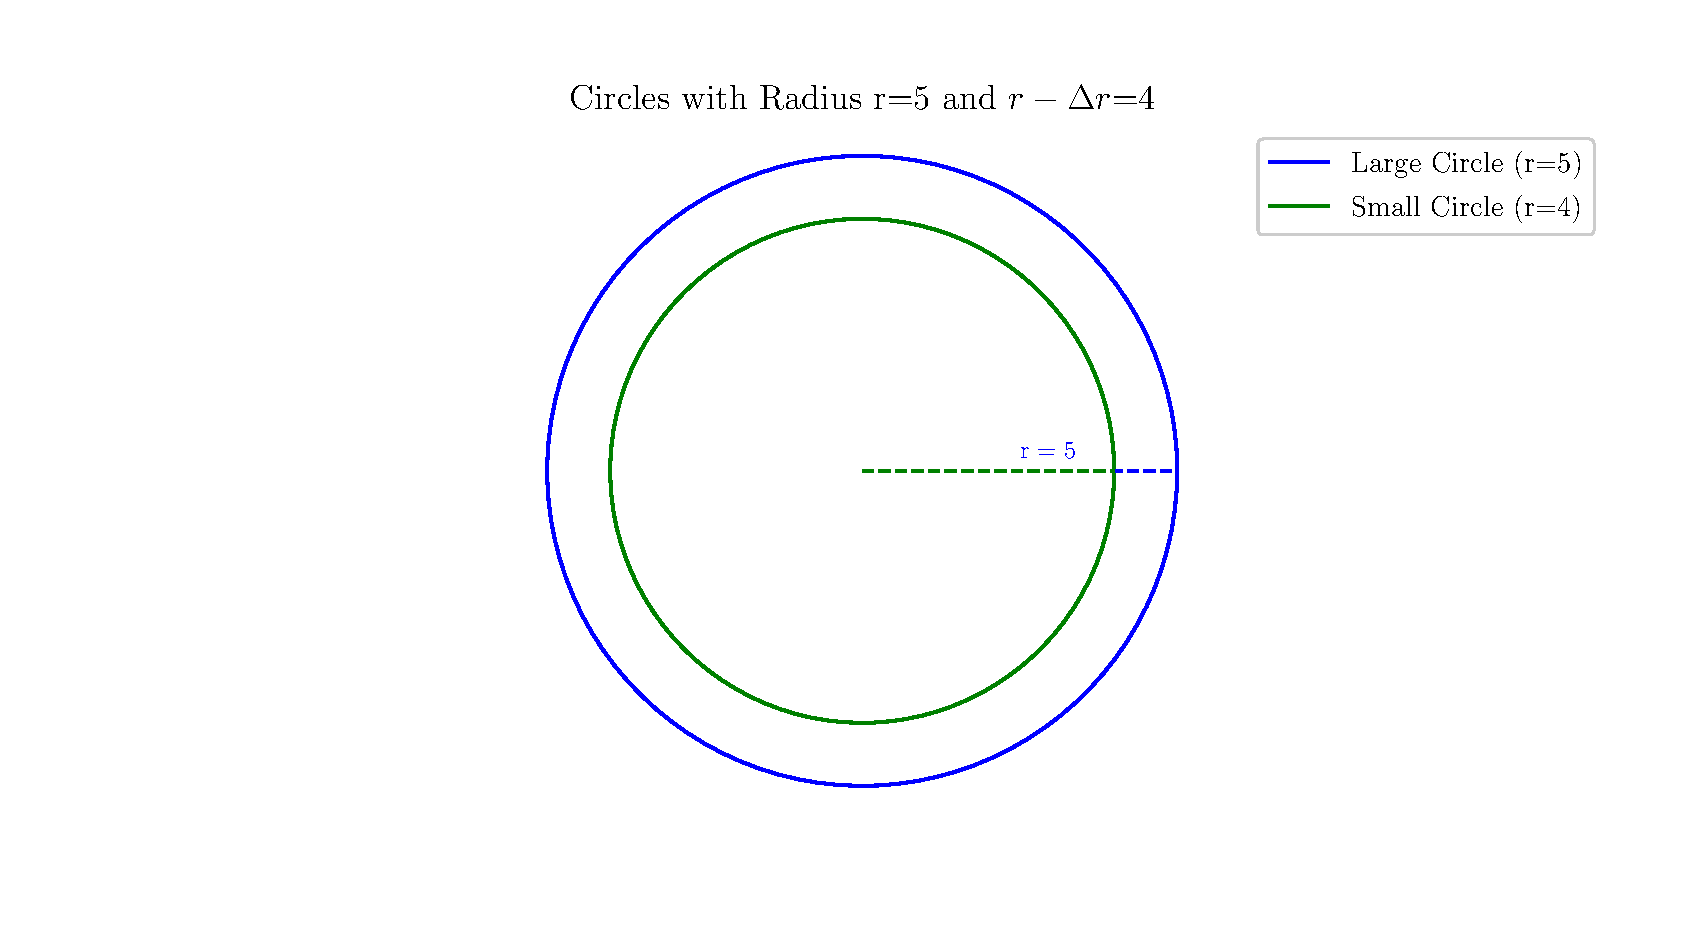
\includegraphics[width=0.8\textwidth]{img/CircleAreaDiverse.eps}
        \caption{细分圆}
    \end{figure}

    如图, 画一个半径$r$的圆, 然后在内部再来一个同圆心但半径比它小$\Delta r$的圆, 这样小圆的半径就是$r-\Delta r$

    两圆的面积相减就得到圆环的面积, 圆环展开是梯形; 如果$\Delta r$趋近于0, 则可以将其看作为长方形, 则有$\Delta S=C\cdot \Delta r=\pi r^2-\pi \left( r-\Delta r \right)^2$

    所以有$$C=\lim_{\Delta r \to 0} \frac{\pi r^2-\pi \left ( r-\Delta r \right )^2 }{\Delta r} $$
    将其化为函数形式, 即为$$C=\lim_{\Delta r \to 0} \frac{f(r)-f(r-\Delta r) }{\Delta r} ,f(r)=\pi r^2$$
    所以$C=f'(r)=2\pi r .\blacksquare$

    \section{\textcolor[rgb]{0.11,0.65,0.52}{P82, P83}}
    \textcolor[rgb]{0.38,0.11,0.2}{牛顿迭代法}的简单介绍.\cite{Newton}

    首先, 选择一个接近函数${\displaystyle f(x)}$零点的${\displaystyle x_{0}}$, 计算相应的${\displaystyle f(x_{0})}$和切线斜率${\displaystyle f'(x_{0})}$(这里${\displaystyle f'}$表示函数${\displaystyle f}$的导数). 然后我们计算穿过点${\displaystyle (x_{0},f(x_{0}))}$并且斜率为${\displaystyle f'(x_{0})}$的直线和${\displaystyle x}$轴的交点的${\displaystyle x}$坐标, 也就是求如下方程的解:$${\displaystyle 0=(x-x_{0})\cdot f'(x_{0})+f(x_{0})}$$
    我们将新求得的点的${\displaystyle x}$坐标命名为${\displaystyle x_{1}}$通常${\displaystyle x_{1}}$会比${\displaystyle x_{0}}$更接近方程${\displaystyle f(x)=0}$的解因此我们现在可以利用${\displaystyle x_{1}}$开始下一轮迭代. 迭代公式可化简为如下所示$${\displaystyle x_{n+1}=x_{n}-{\frac {f(x_{n})}{f'(x_{n})}}}$$

    \section{\textcolor[rgb]{0.11,0.65,0.52}{P87, P99 T13}}
    
    拓展一个\textcolor[rgb]{0.38,0.11,0.2}{三次函数}相关结论.

    三次函数$\displaystyle y=ax^3+bx^2+cx+d,(a\neq 0)$的性质:
    \begin{enumerate}
        \item 单调性: 若$b2-3ac\le 0$, 在$\mathbb{R}$上单调; 若$b2-3ac> 0$, 在$\mathbb{R}$上有三个单调区间;
        \item 对称中心: 关于点$\displaystyle \left( -\frac{b}{3a},f\left( -\frac{b}{3a} \right) \right)$对称, \textcolor[rgb]{0.75,0.17,0.22}{横坐标为导数极值点或二阶导数零点};
        \item 韦达定理: 见前文4.7;
        \item 穿针引线法(奇穿偶不穿): 建议从右边往左边画(好判断正负);
        \item 若找不到可求解方案, 可以选择试根后使用长除法;
    \end{enumerate}

    如图18所示, 函数$y=x^3+2x^2+x+1$在$\mathbb{R}$上有三个单调区间, 其中对称中心$O$点坐标为$\displaystyle O\left ( -\frac{2}{3},f\left ( -\frac{2}{3} \right )  \right ) $, 过这个点作函数切线, 将图像分为4个部分, 有三次函数切线结论:

    \begin{figure}[htbp]
        \centering
        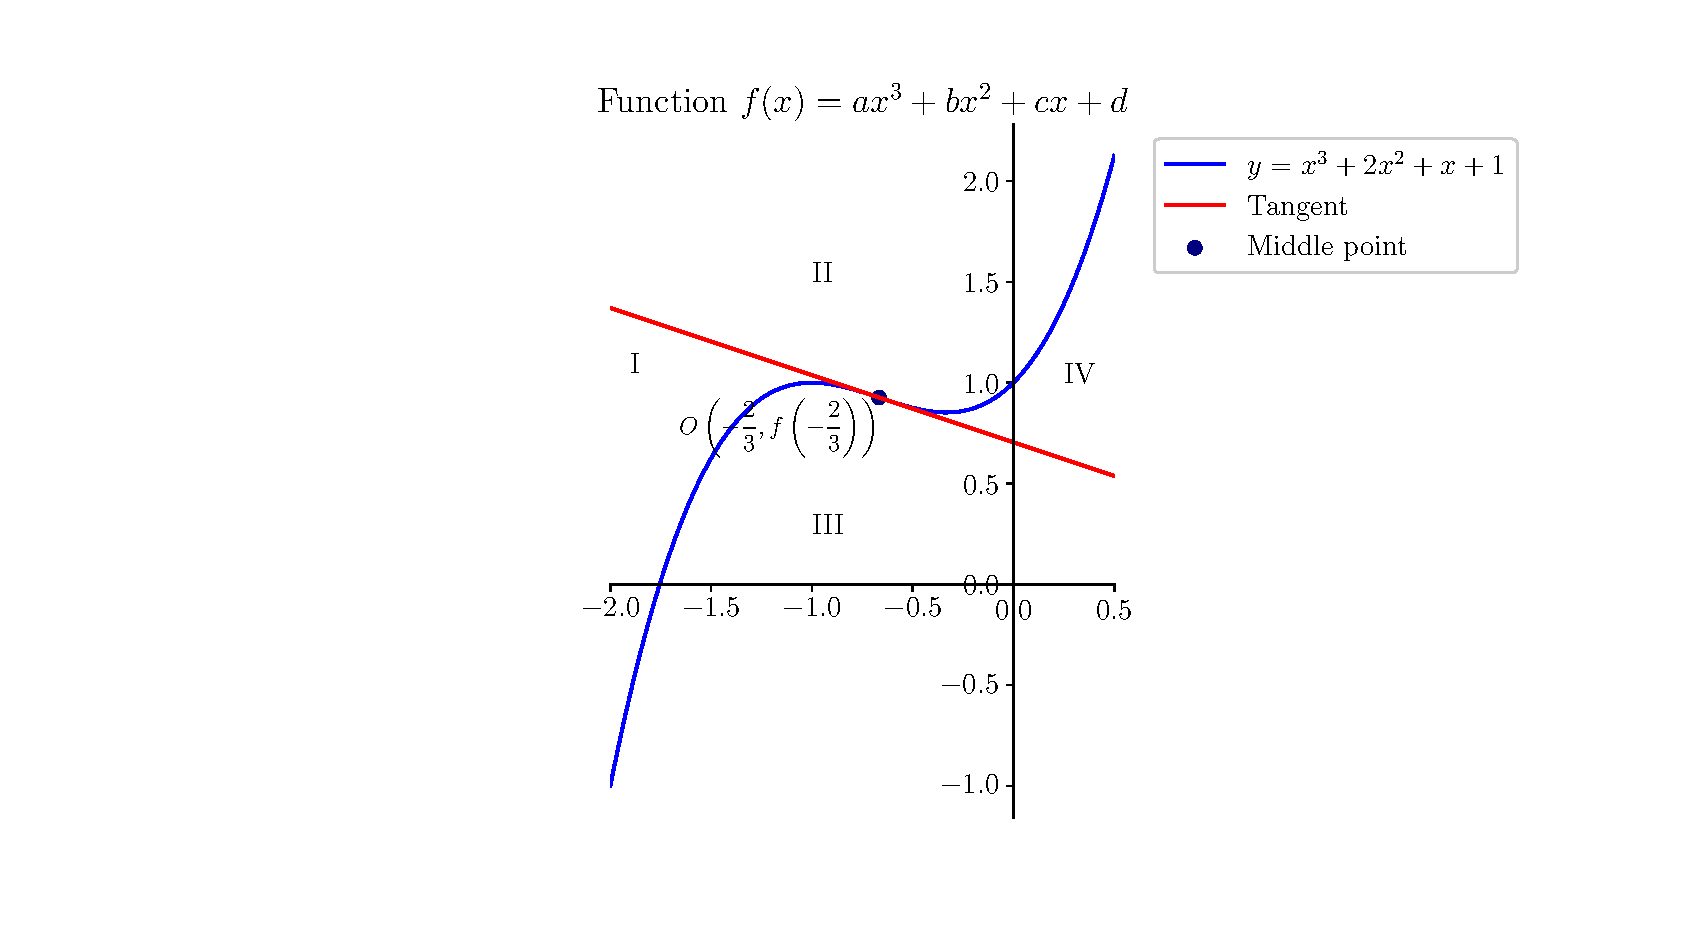
\includegraphics[width=0.8\textwidth]{img/CubicFunction.eps}
        \caption{三次函数切线结论}
    \end{figure}

    \begin{enumerate}
        \item 过I,IV区域内的点做$y$的切线有3条;
        \item 过II,III区域内的点以及对称中心作$y$的切线有1条;
        \item 过$y$上一点或切线(对应图例Tangent)除中心点上一点作切线有2条.
    \end{enumerate}

    \section{\textcolor[rgb]{0.11,0.65,0.52}{P88}}

    此处拓展\textcolor[rgb]{0.38,0.11,0.2}{琴生不等式}和\textcolor[rgb]{0.38,0.11,0.2}{凹凸性}的关系, 由于各种课本对凹凸的概念不同, 故这里均指明是上凸还是下凸, 分别对应英文Convex和Concave.

    对于几何性质的定义, 若在封闭图形上任意取2点作线段能够满足线段上的点均在封闭图形内, 我们称这个图形是凸的; 若在坐标系内, 对于函数$f(x)$上任意两点$(x_1,y_1),(x_2,y_2)$作直线$g(x)=y=kx+b$, 能保证任取一个$x_0\in \left( x_1,x_2 \right)$均有$f(x_0)>g(x_0)$, 则称这个函数$f(x)$在$\left( x_1,x_2 \right)$上凸(Convex). 若$f(x_0)<g(x_0)$, 则称这个函数$f(x)$在$\left( x_1,x_2 \right)$下凸(Concave).
    
    如图19所示, 对于上凸(Convex)函数典例$y=\ln x$, 对其求导可得$$y=\ln x\Longrightarrow y'=\frac{1}{x}\Longrightarrow y''=-\frac{1}{x^2}$$其中二阶导数$y''<0$, 直线函数斜率$y'$单调递减.

    \begin{figure}[htbp]
        \centering
        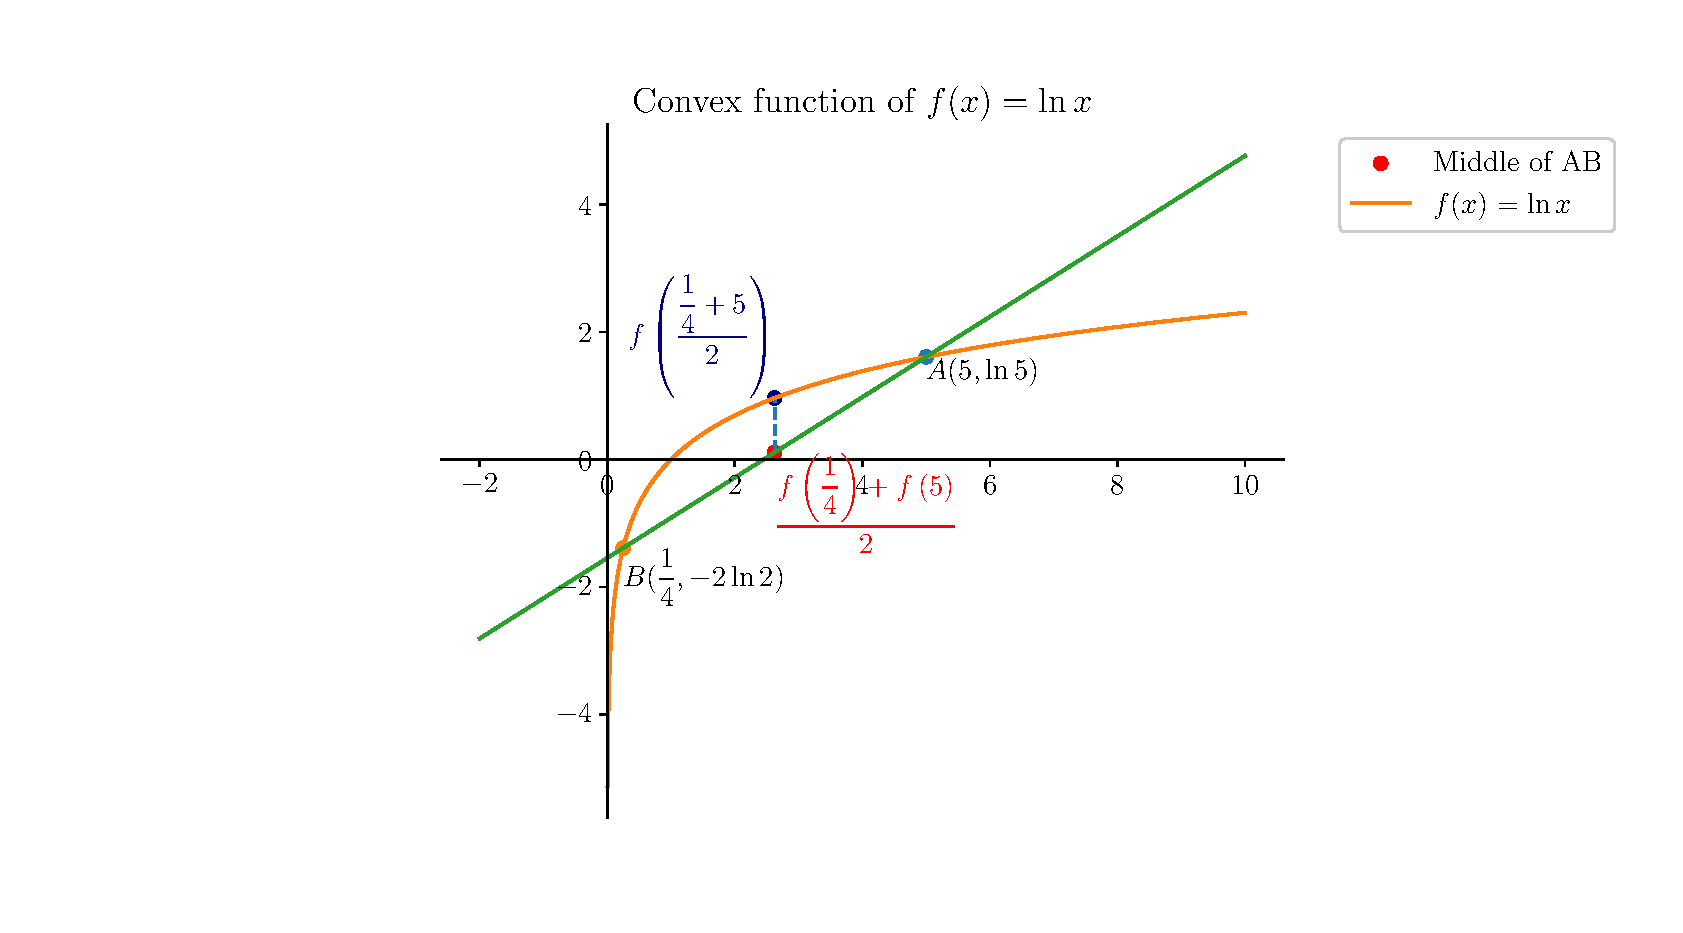
\includegraphics[width=\textwidth]{img/ConvexFunctionIntro.eps}
        \caption{上凸函数$\displaystyle y=\ln x$的性质}
    \end{figure}

    其中有$$f\left( \frac{x_1+x_2}{2} \right)\ge \frac{f\left( x_1 \right)+f\left( x_2 \right)}{2}$$当且仅当$x_1=x_2$取等. 拓展到$n$维$$f\left( \frac{x_1+x_2+x_3+\cdots+x_n}{n} \right)\ge \frac{f(x_1)+f(x_2)+f(x_3)+\cdots+f(x_n)}{n}$$简写为$$f\left( \sum_{i=0}^{n}\frac{x_i }{n} \right)\ge \sum_{i=0}^{n}\frac{f(x_i) }{n}$$当且仅当$x_1=x_2=x_3=\cdots=x_n$取等.

    如图20所示, 对于下凸(Concave)函数典例$y=e^x$, 对其求导可得$$y=e^x\Longrightarrow y'=e^x\Longrightarrow y''=e^x$$其中二阶导数$y''>0$, 直线函数斜率$y'$单调递增.

    \begin{figure}[htbp] 
        \centering
        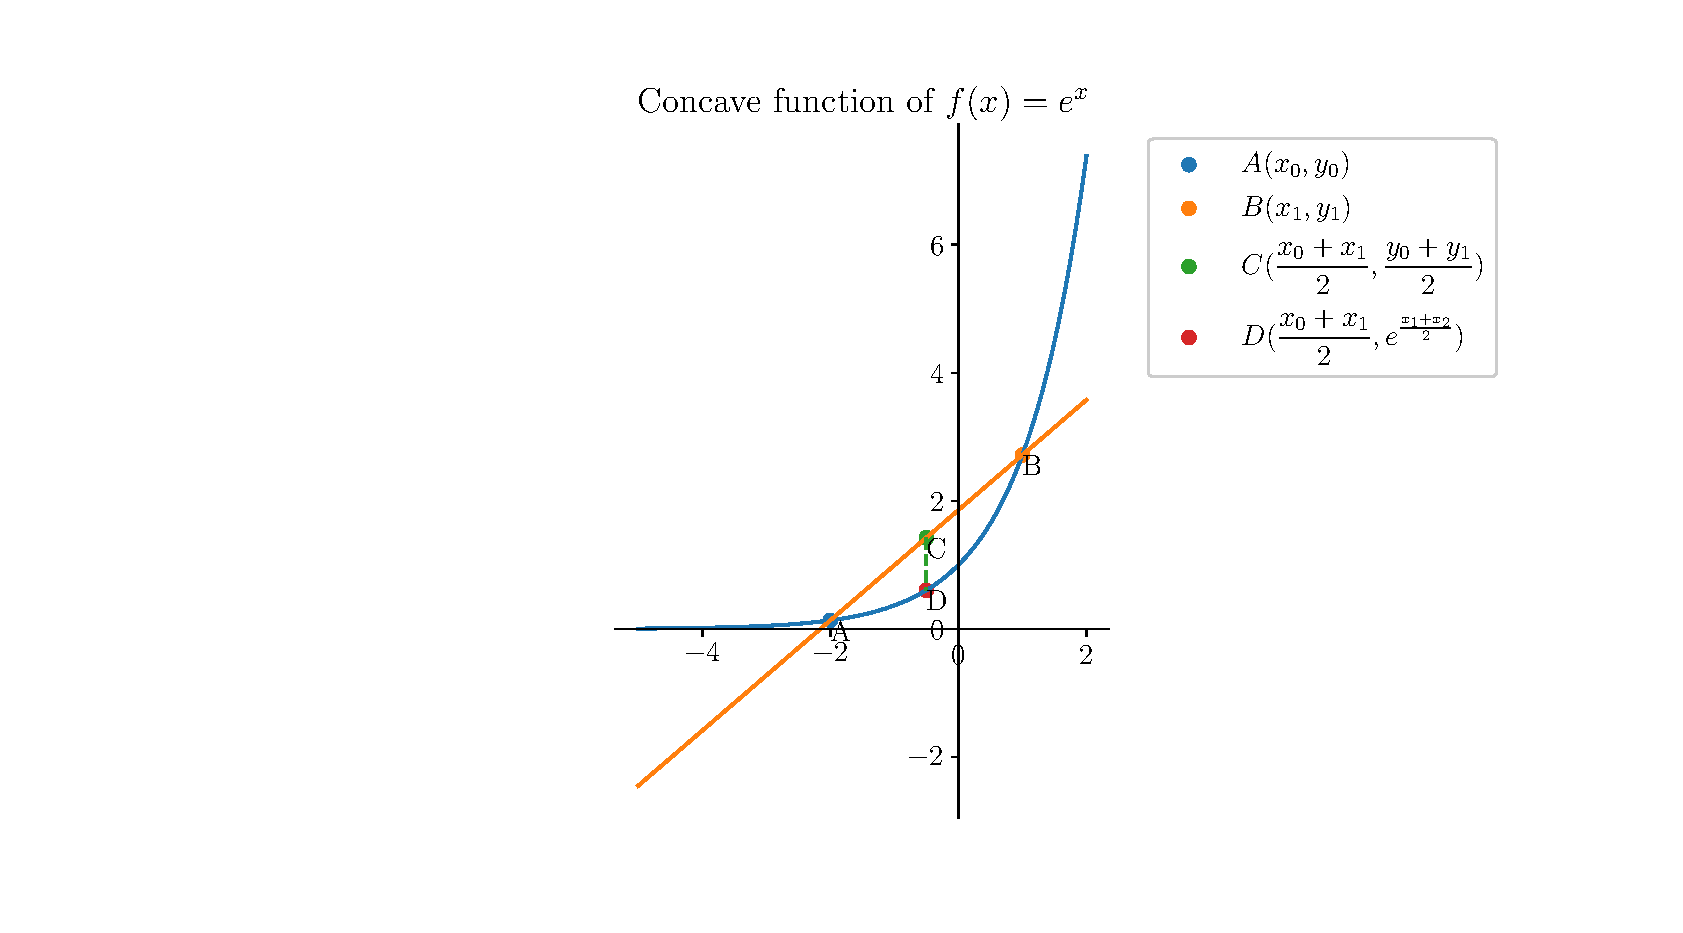
\includegraphics[width=\textwidth]{img/ConcaveFunctionIntro.eps}
        \caption{下凸函数$\displaystyle y=e^x$的性质}
    \end{figure}

    其中有$$f\left( \frac{x_1+x_2}{2} \right)\le \frac{f\left( x_1 \right)+f\left( x_2 \right)}{2}$$当且仅当$x_1=x_2$取等. 拓展到$n$维$$f\left( \frac{x_1+x_2+x_3+\cdots+x_n}{n} \right)\le \frac{f(x_1)+f(x_2)+f(x_3)+\cdots+f(x_n)}{n}$$简写为$$f\left( \sum_{i=0}^{n}\frac{x_i }{n} \right)\le \sum_{i=0}^{n}\frac{f(x_i) }{n}$$当且仅当$x_1=x_2=x_3=\cdots=x_n$取等.

    如果是二维琴生不在中点而是一般的点就有加权形式:
    \begin{enumerate}
        \item 上凸函数: $f\left( ax_1+\left( 1-a \right)x_2 \right)\ge af\left( x_1 \right)+(1-a)f\left( x_2 \right)$
        \item 下凸函数: $f\left( ax_1+\left( 1-a \right)x_2 \right)\le af\left( x_1 \right)+(1-a)f\left( x_2 \right)$
    \end{enumerate}

    \section{\textcolor[rgb]{0.11,0.65,0.52}{P52, T10}}

    本题涉及\textcolor[rgb]{0.38,0.11,0.2}{杨氏不等式}.\cite{Young}

    指出:假设${\displaystyle a}$, ${\displaystyle b}$, ${\displaystyle p}$和${\displaystyle q}$是正实数, 且有${\displaystyle {\frac {1}{p}}+{\frac {1}{q}}=1}$那么:$${\displaystyle ab\leq {\frac {a^{p}}{p}}+{\frac {b^{q}}{q}}}$$等号成立当且仅当${\displaystyle a^{p}=b^{q}}$因为这时${\displaystyle ab=a(b^{q})^{1 \over q}=aa^{p \over q}=a^{p}={a^{p} \over p}+{b^{q} \over q}}$

    证明: 我们知道函数${\displaystyle f(x)=e^{x}}$为下凸函数, 因为它的二阶导数恒为正. 从而我们有$${\displaystyle ab=e^{\ln(a)}e^{\ln(b)}=e^{{1 \over p}\ln(a^{p})+{1 \over q}\ln(b^{q})}\leq {1 \over p}e^{\ln(a^{p})}+{1 \over q}e^{\ln(b^{q})}={a^{p} \over p}+{b^{q} \over q}}$$这里我们使用了下凸函数的一个性质: 对任意$t$, 若${\displaystyle 0<t<1}$则有:$${\displaystyle f(tx+(1-t)y)\leq tf(x)+(1-t)f(y)}$$
    所以有$${\displaystyle ab\leq {\frac {a^{p}}{p}}+{\frac {b^{q}}{q}}}$$成立, 当且仅当${\displaystyle a^{p}=b^{q}}$等号成立.$\blacksquare$

    通过琴生不等式证明杨氏不等式我们发现不等式之间是相互证明的, 读者也可以试着用这些不等式来证明其它的不等式.

    \section{\textcolor[rgb]{0.11,0.65,0.52}{P94,T2,P99,T12}}

    \begin{figure}[htbp] 
        \centering
        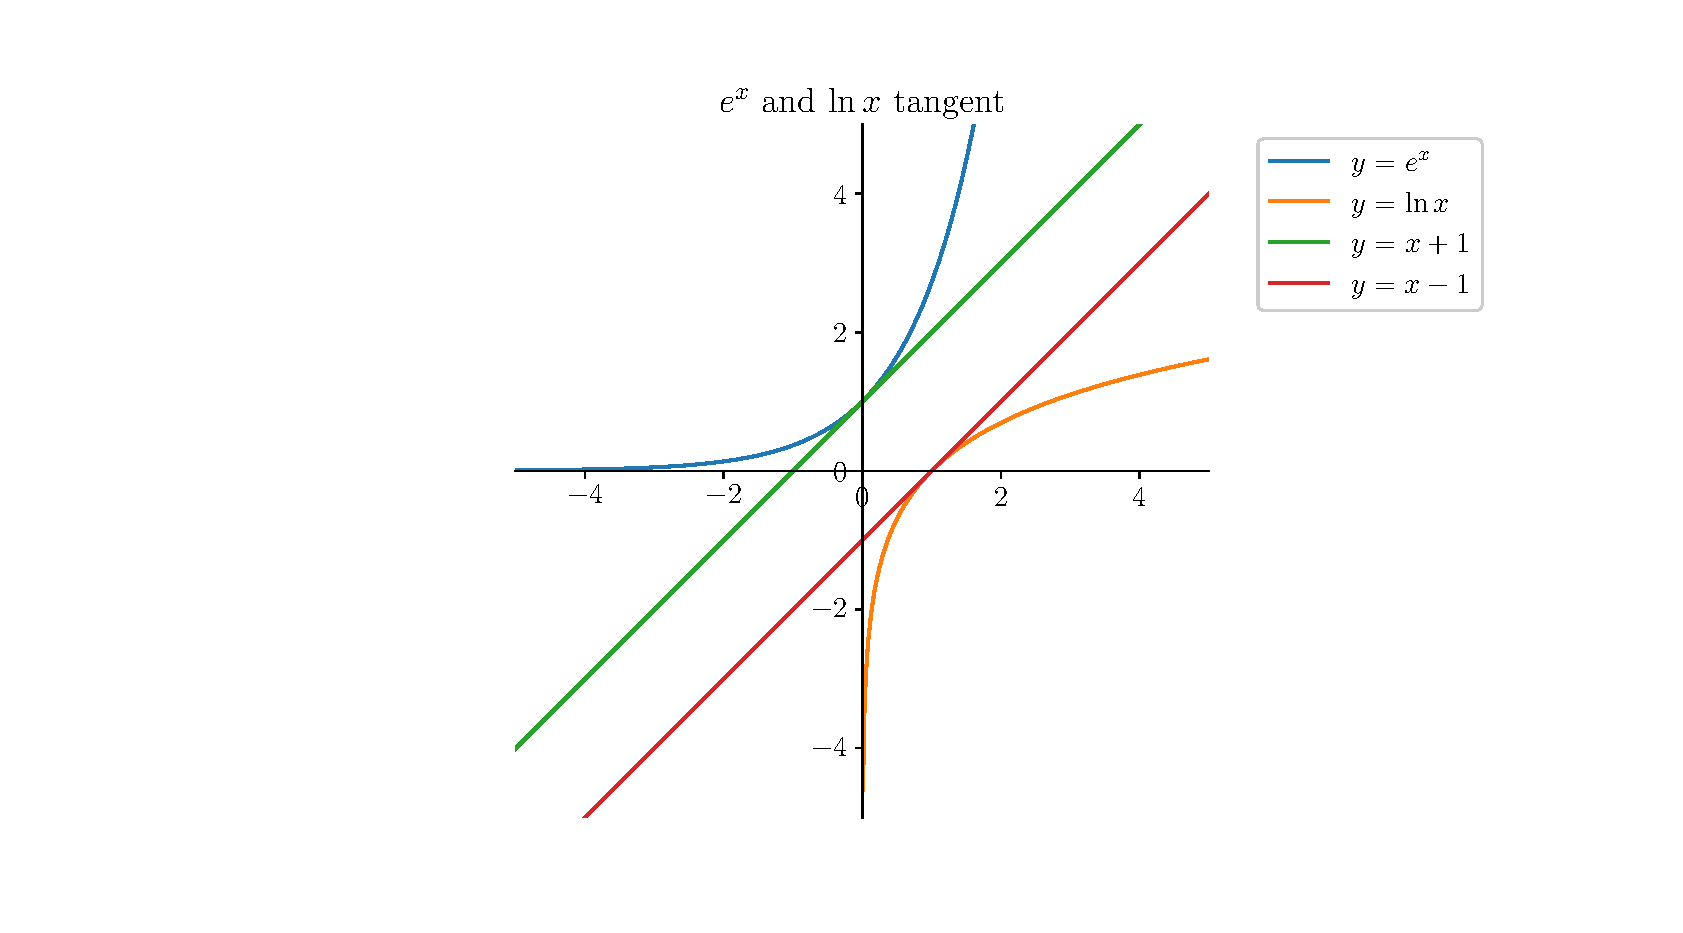
\includegraphics[width=\textwidth]{img/LogExFunction.eps}
        \caption{切线放缩}
    \end{figure}

    \subsection{证明$e^x\ge x+1$}

    \textcolor[rgb]{0.75,0.17,0.22}{作差构造函数}:$f(x)=e^x-x-1$对其求导可得$f'(x)=e^x-1$

    \begin{table}[htbp]
        \centering
        \begin{tabular}{|l|l|l|l|}
        \hline
        $x$     & $(-\infty,0)$ & 0   & $(0,+\infty)$ \\ \hline
        $f'(x)$ & $<0$          & 0   & $>0$          \\ \hline
        $f(x)$  & 单调递减          & 极小值 & 单调递增          \\ \hline
        \end{tabular}
    \end{table}
    所以$$f(x)\ge f(0)=0\Longrightarrow e^x-x-1\ge 0\Longrightarrow e^x\ge x+1.\blacksquare$$

    \subsection{证明$\ln x\le x-1$}

    \textcolor[rgb]{0.75,0.17,0.22}{作差构造函数}:$f(x)=x-1-\ln x$对其求导可得$\displaystyle f'(x)=1-\frac{1}{x}$

    \begin{table}[htbp]
        \centering
        \begin{tabular}{|l|l|l|l|}
        \hline
        $x$     & $(0,1)$ & 1   & $(1,+\infty)$ \\ \hline
        $f'(x)$ & $<0$    & 0   & $>0$          \\ \hline
        $f(x)$  & 单调递减    & 极小值 & 单调递增          \\ \hline
        \end{tabular}
        \end{table}

    所以$$f(x)\ge f(1)=0\Longrightarrow x-1-\ln x\ge 0\Longrightarrow \ln x\le x-1.\blacksquare$$

    \section{\textcolor[rgb]{0.11,0.65,0.52}{P97, 练习一}}

    \begin{boxB}
        证明$\displaystyle \sin x<x<\tan x,x\in\left( 0,\frac{\pi}{2} \right)$
    \end{boxB}

    \subsection{求导法}

    先证明左侧:$x-\sin x>0$, 令$f(x)=x-\sin x$, $f'(x)=1-cos x>0,f(x)>f(0)=0$.

    再证明右侧:$\tan x-x>0$, 令$f(x)=\tan x-x$, $\displaystyle f'(x)=\frac{1}{\cos^2x}-1>0,f(x)>f(0)=0$.$\blacksquare$

    \begin{figure}[htbp] 
        \centering
        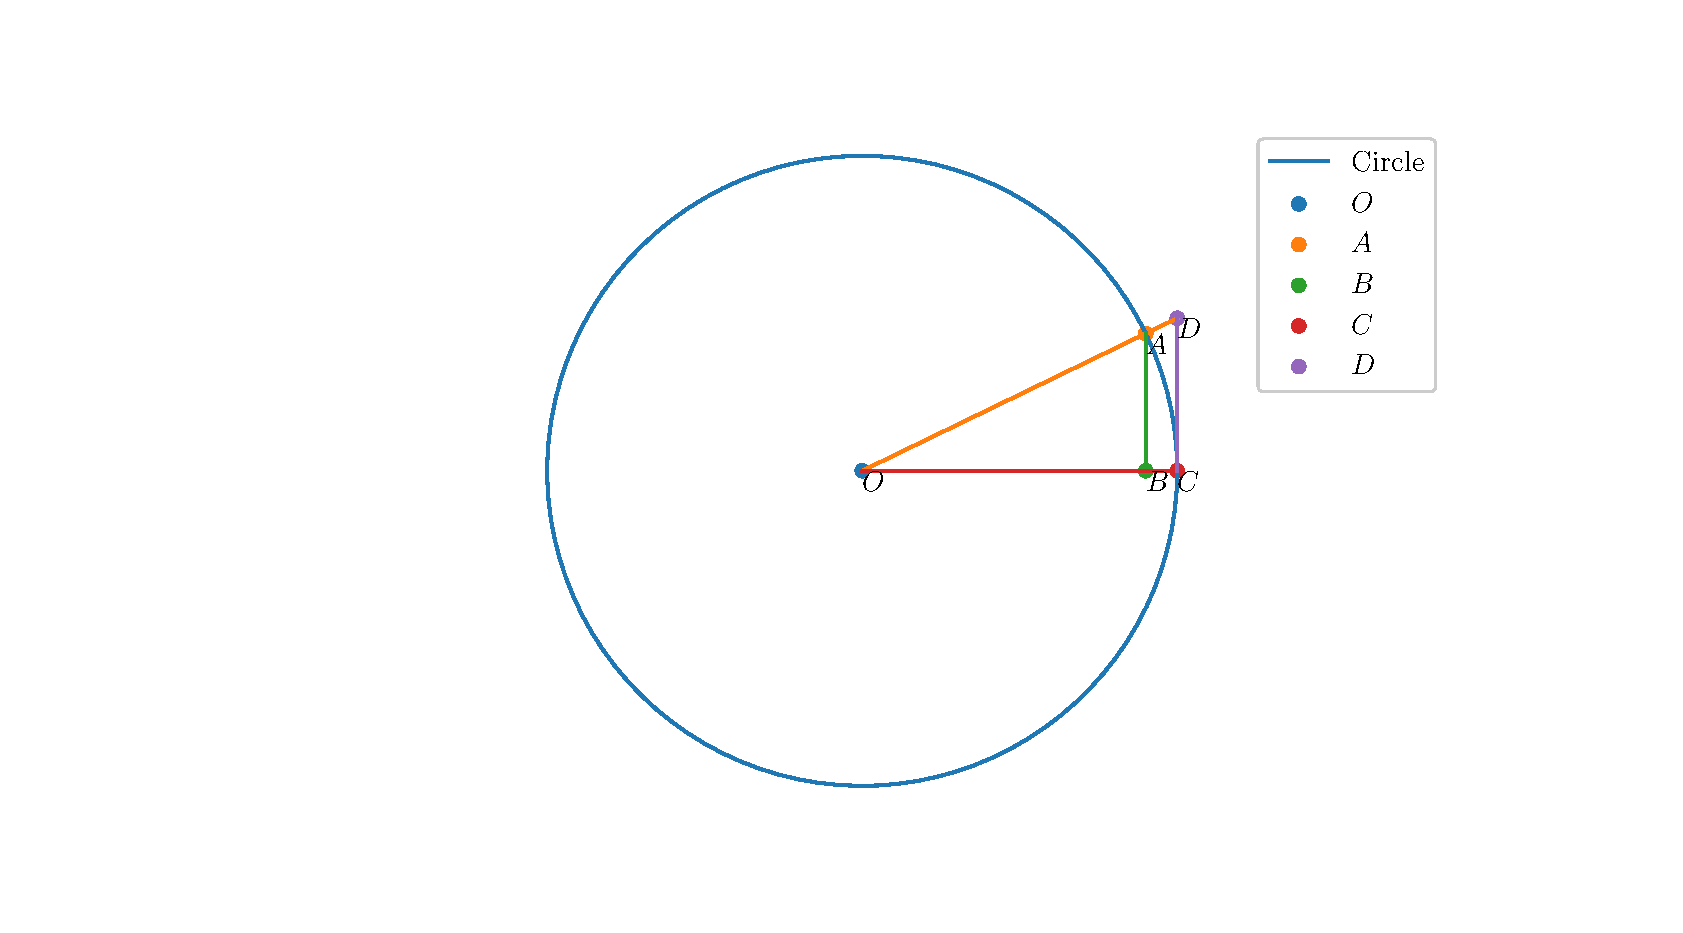
\includegraphics[width=\textwidth]{img/CircleSinTan.eps}
        \caption{几何法}
    \end{figure}

    \subsection{几何法}

    如图22所示: 做单位圆(半径为1),设$OC$与$OC$夹角为$\displaystyle x\in\left( 0,\frac{\pi}{2} \right)$

    由图$\displaystyle \sin x=\frac{AB}{r}=AB,\overset{\frown }{AB}=xr$, 由此可知$\sin x<x$

    又有$\displaystyle \tan x=\frac{DC}{r}=DC$有面积关系$S_{\text{扇形AOC}}<S_{\triangle DOC}$

    又$\displaystyle S_{\triangle DOC}=\frac{1}{2}OC\cdot CD\frac{\tan x}{2}$, $\displaystyle S_{\text{扇形}AOC}=\frac{1}{2}xr^2=\frac{x^2}{2}$

    由$S_{\text{扇形}}<S_{\triangle DOC}$可得$\displaystyle x<\tan x,x\in\left( 0,\frac{\pi}{2} \right)$

    \subsection{第一类重要极限}
    由此我们可以拓展一个\textcolor[rgb]{0.38,0.11,0.2}{第一类重要极限}

    刚刚已经证明$\sin x<x<\tan x$在$\displaystyle x\in\left( 0,\frac{\pi}{2} \right)$上成立, 此时若等式均同除以$\sin x$, 我们可以得到:$$1<\frac{x}{\sin x}<\frac{1}{\cos x}$$对上式取倒数, 我们可以得到$$\cos x<\frac{\sin x}{x}<1$$此时$\displaystyle \frac{\sin x}{x}$的范围已经被固定在$\left( \cos x,1 \right)$, 若让$x\rightarrow 0$此时有$$\lim_{x \to 0} \cos x=1$$而不等式右边就是1, 故由于\textcolor[rgb]{0.75,0.17,0.22}{夹逼准则}$$\lim_{x \to 0} \frac{\sin x}{x}=1 $$

    \chapter{选择性必修三}

    \section{\textcolor[rgb]{0.11,0.65,0.52}{P39}}
    \textcolor[rgb]{0.38,0.11,0.2}{杨辉三角}第$n$行是$(a+b)^n$的展开式的二项式系数, 第$n$行第$r$个数可以表示为$C_n^{r-1}$.

    \begin{table}[htbp]
        \centering
        \begin{tabular}{lllllllll}
          &   &   & 1 &   & 1 &   &   &   \\
          &   & 1 &   & 2 &   & 1 &   &   \\
          & 1 &   & 3 &   & 3 &   & 1 &   \\
        1 &   & 4 &   & 6 &   & 4 &   & 1 \\
        \end{tabular}
        \end{table}
    \begin{center}
        $\cdots$
    \end{center}
    
    杨辉三角的性质:

    \begin{enumerate}
        \item 第$n$行的数字和为$2^n$, $\left( C_n^0+C_n^1+C_n^2+\cdots+C_n^n=(1+1)^n \right)$;
        \item $C_n^r=C_{n-1}^{r-1}+C_{n-1}^r$;
        \item 斜线之和满足斐波那契数列.
    \end{enumerate}

    \section{\textcolor[rgb]{0.11,0.65,0.52}{P51, P53 $\sim$ P55}}
    贝叶斯公式: 设$A_1,A_2,A_n$, 是一组两两互斥的事件, $A_1\cup A_2\cup \cdots \cup A_n=\Omega$, $P(A_i)>0,i=1,2,3,\cdots,n$, 则对任意的事件$B\subseteq \Omega,P(B)>0$, 有:$$P\left( A_i\Big|B \right)=\frac{P\left( A_i \right)P\left( B\Big|A_i \right)}{P(B)}=\sum_{k=1}^{n} \frac{P(A_i)P(B|A_i)}{P(A_k)P(B \Big |A_k)},i=1,2,3,\cdots,n$$

    \textcolor[rgb]{0.38,0.11,0.2}{三门问题}: 在一个抽奖游戏中有三个外观相同的门, 主持人在三扇门中随机放1辆豪车(中奖)和2个山羊(没中奖), 此时主持人让抽奖人在三扇门选择其中一个, 接着主持人从你没选的两扇门中选择一个山羊的门, 此时主持人给你一次更换的机会, 你会坚持之前的抉择还是改成另一个呢?

    设$A_1,A_2,A_3$;表示3个门有奖品的3种情况; $B_1,B_2,B_3$, 表示主持人会打开的门的3种情况. 此时$\displaystyle P(A_1)=P(A_2)=P(A_3)=\frac{1}{3}$,如果我选1, 主持人在2,3中挑选, 我们对主持人开2号门进行研究; 其中$\displaystyle P\left( B_2\Big|A_1 \right)=\frac{1}{2},P\left( B_2\Big|A_2 \right)=0,P\left( B_2\Big|A_3 \right)=1$;全概率: $$P\left( B_2 \right)=\sum_{i=1}^{3} P(A_i)P\left ( B_2\Big |A_i \right ) =\frac{1}{3}\times \frac{1}{2} +\frac{1}{3}\times 0+\frac{1}{3}\times 1=\frac{1}{2} $$贝叶斯:$$P\left( A_1\Big|B_2 \right)\frac{P(A_1)P\left( B_2\Big|A_1 \right)}{P(B_2)}=\frac{1}{3};P\left( A_3\Big|B_2 \right)\frac{P(A_3)P\left( B_2\Big|A_3 \right)}{P(B_2)}=\frac{2}{3}$$
    \section{\textcolor[rgb]{0.11,0.65,0.52}{P91, T10}}
    这里涉及\textcolor[rgb]{0.38,0.11,0.2}{马尔可夫链}.
    
    \begin{boxB}
        甲, 乙, 丙三人相互做传球训练, 第1次由甲将球传出, 每次传球时, 传球者都等可能地将球传给另外两个人中的任何一人, 求$n$次传球后球在甲手中的概率.
    \end{boxB}

    记$P_n$表示第$n$次传球后球在甲手中, 其中$P_1=0$(因为甲第一次传出去)如果$n+1$次回到甲手中, 此时第$n$次就不可能在甲手中了, 此时\textcolor[rgb]{0.75,0.17,0.22}{第$n$次不在甲手中的概率是$(1-P_n)$}

    此时第$n$次可能有四种情况: 乙$\rightarrow$甲, 乙$\rightarrow$丙, 丙$\rightarrow$甲, 丙$\rightarrow$乙, 又该过程中情况等概率, 则$n+1$次到甲手中概率是, 由分步计数乘法可知:$$P_{n+1}=\frac{1}{2}\left( 1-P_n \right)=\frac{1}{2}-\frac{1}{2}P_n\Longrightarrow P_{n+1}-\frac{1}{3}=-\frac{1}{2}\left( P_n-\frac{1}{3} \right)$$由此可得$$P_n=\frac{1}{3}-\frac{1}{3}\left( -\frac{1}{2} \right)^{n-1}$$
    本质考察数列与概率的结合, 实际上涉及\textcolor[rgb]{0.38,0.11,0.2}{马尔科夫链}的相关知识. 

    \begin{thebibliography}{99}
        \bibitem{complex}Incidence bounds with Möbius hyperbolae in positive characteristic, Misha Rudnev, James Wheeler, Wed, 21 Apr 2021 13:47:42 UTC
        \bibitem{Fibonacci}Wikipedia contributors. "Fibonacci sequence." Wikipedia, The Free Encyclopedia. Wikipedia, The Free Encyclopedia, 15 Oct. 2024. Web. 19 Oct. 2024.
        \bibitem{induction}Wikipedia contributors. "Mathematical induction." Wikipedia, The Free Encyclopedia. Wikipedia, The Free Encyclopedia, 9 Sep. 2024. Web. 19 Oct. 2024.
        \bibitem{Newton}Wikipedia contributors. "Newton's method." Wikipedia, The Free Encyclopedia. Wikipedia, The Free Encyclopedia, 14 Oct. 2024. Web. 20 Oct. 2024.
        \bibitem{Young}Hardy, G. H.; Littlewood, J. E.; and Pólya, G. "A Theorem of W. H. Young." §8.3 in Inequalities, 2nd ed. Cambridge, England: Cambridge University Press, pp. 198-200, 1988.
    \end{thebibliography}

\end{document}
